%% ---------------------------------------------
\documentclass[preprint,3p,12pt,english]{elsarticle}

\usepackage{subfigure}
\usepackage{amssymb}
\usepackage{amsmath}
\usepackage{natbib}
\usepackage{color}
\usepackage{hyperref}
\usepackage{pifont}
\usepackage{parskip}
\usepackage{fixltx2e}
\usepackage{array}
\bibliographystyle{unsrt}
\usepackage[normalem]{ulem}
\usepackage{caption}
%\usepackage[T1]{fontenc}
\usepackage[utf8]{inputenc}
\usepackage{babel}
\usepackage[font=small,labelfont=bf]{caption}
\usepackage[switch,pagewise, modulo]{lineno}
\newcommand{\margin}[1]{\textcolor{red}{#1}}
\newcommand{\out}[1]{\textcolor{green}{#1}}
\usepackage{float}
\usepackage{nomencl}
\usepackage{ifthen}
\renewcommand{\nomgroup}[1]{%
  \ifthenelse{\equal{#1}{R}}{\item[\textbf{Roman Symbols}]}{%
    \ifthenelse{\equal{#1}{G}}{\item[\textbf{Greek Symbols}]}{%
      \ifthenelse{\equal{#1}{A}}{\item[\textbf{Abbreviations}]}{%
        \ifthenelse{\equal{#1}{S}}{\item[\textbf{Subscripts}]}{%
          \ifthenelse{\equal{#1}{U}}{\item[\textbf{Superscripts}]}{}
        }% matches mathematical symbols
      }% matches Subscripts
    }% matches Abbreviations
  }% matches Greek Symbols
}% matches Roman Symbols
\renewcommand*{\nompreamble}{\footnotesize}
\usepackage{footnote}
 \makenomenclature
\renewcommand{\nomname}{Nomenclature}
\newcommand{\degree}{\ensuremath{^\circ}}
\renewcommand{\arraystretch}{1.5}
\usepackage{framed} % Framing content
\usepackage{multicol} % Multiple columns environment
\renewcommand*\nompreamble{\begin{multicols}{2}}
\renewcommand*\nompostamble{\end{multicols}}
\captionsetup[table]{skip=3pt}
\makeatletter
\newcommand*{\rom}[1]{\expandafter\@slowromancap\romannumeral #1@}
\makeatother
\newcommand{\nomunit}[1]{%
\renewcommand{\nomentryend}{\hspace*{\fill}#1}}
\biboptions{square,compress}
%\usepackage[noheads,nomarkers]{endfloat}
\def\imagetop#1{\vtop{\null\hbox{#1}}}
\def\imagecenter#1{\raisebox{-0.5\height}{#1}}
\usepackage{amsfonts}
\newcommand{\overbar}[1]{\mkern 1.5mu\overline{\mkern-1.5mu#1\mkern-1.5mu}\mkern 1.5mu}
%\usepackage[showframe]{geometry}
\usepackage[ampersand]{easylist}
\ListProperties(Hide=100, Hang=true, Progressive=3ex, Style*=-- ,
Style2*=$\bullet$ ,Style3*=$\circ$ ,Style4*=\tiny$\blacksquare$ )
\DeclareUnicodeCharacter{00A0}{ }

 \journal{Journal of Atmospheric Science}
\setlength{\parindent}{2em}

\geometry{left=1.2in, right=1.2in, top=1in, bottom=1in}

%%%%%%%%%%%%%%%%%%%%%%%%%%%%%%%%%%%%%%%%%%%%%%%%%%%%%%%%%%%%%%%%%%%%%%%%%%%%%%%%%%%%%%%%%%%%%%%%%%%%%

\begin{document}
\footskip=0.5in % 
\begin{frontmatter}

\title{Predicting Thermal Comfort in Outdoor Urban Environments: A New Numerical Model for Standard Effective Temperature}

\author[rvt]{J. Fan \corref{cor1}}
\ead{jif015@ucsd.edu}
\author[rvt]{N. Nazarian}
\ead{nenazarian@ucsd.edu}
\author[rvt]{J. Kleissl}
\ead{jkleissl@ucsd.edu}

\cortext[cor1]{Corresponding author, Tel.:(+01)480-284-9347 }
\address[rvt]{Mechanical and Aerospace Engineering, University of California, San Diego, 9500 Gilman Dr. 0411, La Jolla, CA 92093-0411}


%%%%%%%%%%%%%%%%%%%%%%%%%%%%%%%%%%%%%%%%%%%%%%%%%%%%%%%%%%%%%%%%%%%%%%%%%%%%%%%%%%%%%%%%%%%%%%%%%%%%%

\begin{abstract}
Rapid urbanization has spurred major health concerns on heat stress in densely built-up areas. An understanding of outdoor thermal comfort is critical for improving people-centric urban design and mitigating heat island effects. Thermal comfort describes human thermal sensation, which is analyzed through comprehensive indices such as the Standard Effective Temperature (SET). This study introduces an improved method of predicting the spatial variation of Standard Effective Temperature by employing a detailed Computational Fluid Dynamics (CFD) model. Spatial distributions of thermal comfort are evaluated at the pedestrian level (1.5 m above ground) in an idealized urban area and a clear summer day in San Diego, California. The CFD provides flow field coupled with heat transfer as input variables for the SET calculation. Thermal comfort is then calculated with a detailed model of mean radiant temperature that is improved by analyzing the visibility of urban surfaces, the sky view factor, and shading effects from buildings. With the developed model, the sensitivity study shows that urban density, wind patterns, and solar position concurrently influence thermal comfort. Because of these concurrent influences, design factors can be optimized for outdoor thermal comfort. 


\textbf{Keywords:} Computational Fluid Dynamics, Mean Radiant Temperature, Outdoor Thermal Comfort, Standard Effective Temperature, Urban Microclimate 

\end{abstract}
\end{frontmatter}
%%%%%%%%%%%%%%%%%%%%%%%%%%%%%%%%%%%%%%%%%%%%%%%%%%%%%%%%%%%%%%%%%%%%%%%%%%%%%%%%%%%%%%%%%%%%%%%%%%%%%
\section{Introduction}

In 2008, the global urban population exceeded the rural population for the first time in human history \cite{desa2014world}. The 2014 UN World Urbanization Prospects report further predicts that the proportion of urban dwellers will increase to two-thirds globally by 2050. One major environmental consequence of urbanization is the Urban Heat Island (UHI), which refers to the relative rise of temperature in densely built areas. \cite{kim1992urban, oke1981canyon, oke1973city, bornstein1968observations}. The UHI is responsible for significant public health concerns due to increased heat stress in densely built areas \cite{tan2010urban, lo2003land, mavrogianni2011comfort}. The human response to airflow, humidity, and radiation exposure is described by outdoor thermal comfort \cite{pickup_outdoor_2000}. More accurate methods of outdoor thermal comfort evaluation and prediction are needed in order to address the rise of extreme weather events around the world \cite{katz1992extreme, goswami2006increasing} and growing concerns about urban sustainability. This can inform designers and architects on the environmental impacts of their design, and help to propose strategies for mitigating UHI and the ensuing health concerns.

Thermal comfort has both been monitored and modelled in several different studies. Field studies combine microclimate measurements and pedestrian interviews in order to observe thermal comfort in real urban environments \cite{chow_assessment_2016,lin_thermal_2009,nikolopoulou2001thermal}. In Hong Kong, Niu et al. \cite{niu_new_2015} found that thermal comfort varied significantly within a university campus and observed the influence of microclimate and building design on thermal comfort.  While field studies verify high spatial variance of thermal comfort and prove that better urban design can improve thermal comfort, they fall short of accurately identifying controllable variables in order to inform designers. Conversely, numerical simulations can address such parameters by predicting thermal comfort. 

There are three popular thermal comfort models: the Fanger comfort model \cite{fanger1967calculation, fanger1972thermal}, the Pierce two-nodes model \cite{gagge1971effective} and the KSU two-nodes model \cite{azer1977}. The Fanger comfort model assumes that the heat exchange between human body and thermal environment is in steady state. Conversely, the Pierce two-nodes model and KSU two-nodes model emphasize the dynamic heat exchange between human body and thermal environment. These thermal comfort models are the basis for different indexes used to quantify thermal comfort \cite{epstein2006thermal,honjo2009thermal}. For example, the Predicted Mean Vote (PMV) was developed based on the Fanger comfort model. The PMV is an empirically based index, and is more applicable for field measurements of thermal comfort \cite{ye2003new}.  Another common thermal comfort index is the Physiological Equivalent Temperature (PET), which is based on a different heat balance model, the Munich energy balance model for individuals (MEMI) \cite{honjo2009thermal}. In this study, thermal comfort predictions are calculated using Standard Effective Temperature (SET), which is an index developed from the Pierce two-nodes model \cite{oohori1984comparison}.  SET is a comprehensive metric that integrates the influences of air temperature, wind velocity, humidity and radiation on the thermal sensation. As it successfully relates all the environmental variables with a person’s thermal experience, it is one of the most commonly used thermal comfort indices \cite{ye2003new}. 

Previous thermal comfort simulations have examined the effects of solar access, shading, wind patterns, vegetation and other parameters \cite{andreou_thermal_2013, acero_comparison_2015}. Ali-Toudert and Mayer used numerical modelling to examine the effects of shading from different urban canyon forms and vegetation patterns in improving thermal comfort \cite{ali2006effects,ali-toudert_effects_2007}. However, many of such simulations are limited in accuracy and in resolution due to simplifications in modelling pedestrian exposure to radiation. Among the factors influencing thermal comfort, radiant heat transfer is one of the most important parameters in human thermal sensation. Accordingly, one major variable in SET calculation is mean radiant temperature ($T_{mrt}$), which accounts for pedestrian exposure to longwave and shortwave radiation. Due to the complexity of mean radiant temperature calculations, simplified models are frequently used in thermal comfort studies. For example, in the simulation done by Ali-Toudert and Mayer, $T_{mrt}$ is assumed to be equal to $T_{air}$. Several different methods for simulating $T_{mrt}$ in outdoor environments have been developed, including ENVI-met 3.1 \cite{bruse2004envi}, Rayman 1.2 \cite{matzarakis2007modelling}, CityComfort+ \cite{huang2014citycomfort+} and SOLWEIG 2.2 \cite{lindberg2008solweig}. However, these $T_{mrt}$ modelling methods have different limitations on accuracy or spatial prediction ability. \jan{Avoid broad statements like ``not user friendly''. If one of the reviewers was an ENVI-met developer it may backfire. Specific criticisms and those that are backed up by the literature are ok as we do need to justify the advantage of our model.}ENVI-met is not user friendly, and requires users to manually transfer topography and vegetation pixels with each simulation. It is also computationally demanding and difficult to use on common desktop computers. Some studies have also questioned the validity of ENVI-met results in comparison to field measurements \cite{toudertdependence}. Rayman, on the other hand, is more user-friendly but can only simulate the MRT at one position per time. Moreover, it does not account for reflected solar radiation, which results in low accuracy specifically for high albedo surfaces \cite{thorsson2007different}. SOLWEIG 2.2 has been shown to sacrifice accuracy due to a simplified radiation formula \cite{lindberg2008solweig}. CityComfort+ is still under development, and is limited in accuracy because it simplifies the calculation of longwave atmospheric radiation \cite{huang2014citycomfort+}.  Thus, an accurate calculation of $T_{mrt}$ in a three-dimensional geometry substantially complicates SET prediction in outdoor environments.

The objective of this study is to develop a comprehensive and accurate method to model thermal comfort, by analyzing different factors of thermal comfort at high spatial resolution, and incorporating them into SET calculations. The main contribution is the development of a more comprehensive $T_{mrt}$ model as well as including the detailed CFD data that allows for the spatial representation of the SET. SET distributions are calculated using input parameters from the CFD simulation provided by Nazarian and Kleissl \cite{nazarian2014effects, nazarian2015cfd}. The CFD simulation is supplemented with an enhanced model of pedestrian radiant temperature, as explained in Section 2.  Additionally, the sensitivity of SET to several design and climate elements is evaluated and compared in Section 3. Lastly, conclusions and future implications are presented in Section 4. 

This paper integrates several advanced urban physics models into thermal comfort simulation, such as CFD simulation, MRT modeling, and SET calculation. This method can be further developed and used to analyze thermal comfort of a real configuration of the 3D urban environment for a more faithful prediction of thermal comfort distribution. An overview of the research context and the enhanced model set-up is visualized as a flow chart in Fig. \ref{Fig.Visibility}:
\begin{figure}[H]
\graphicspath{ {image/} }
\centerline{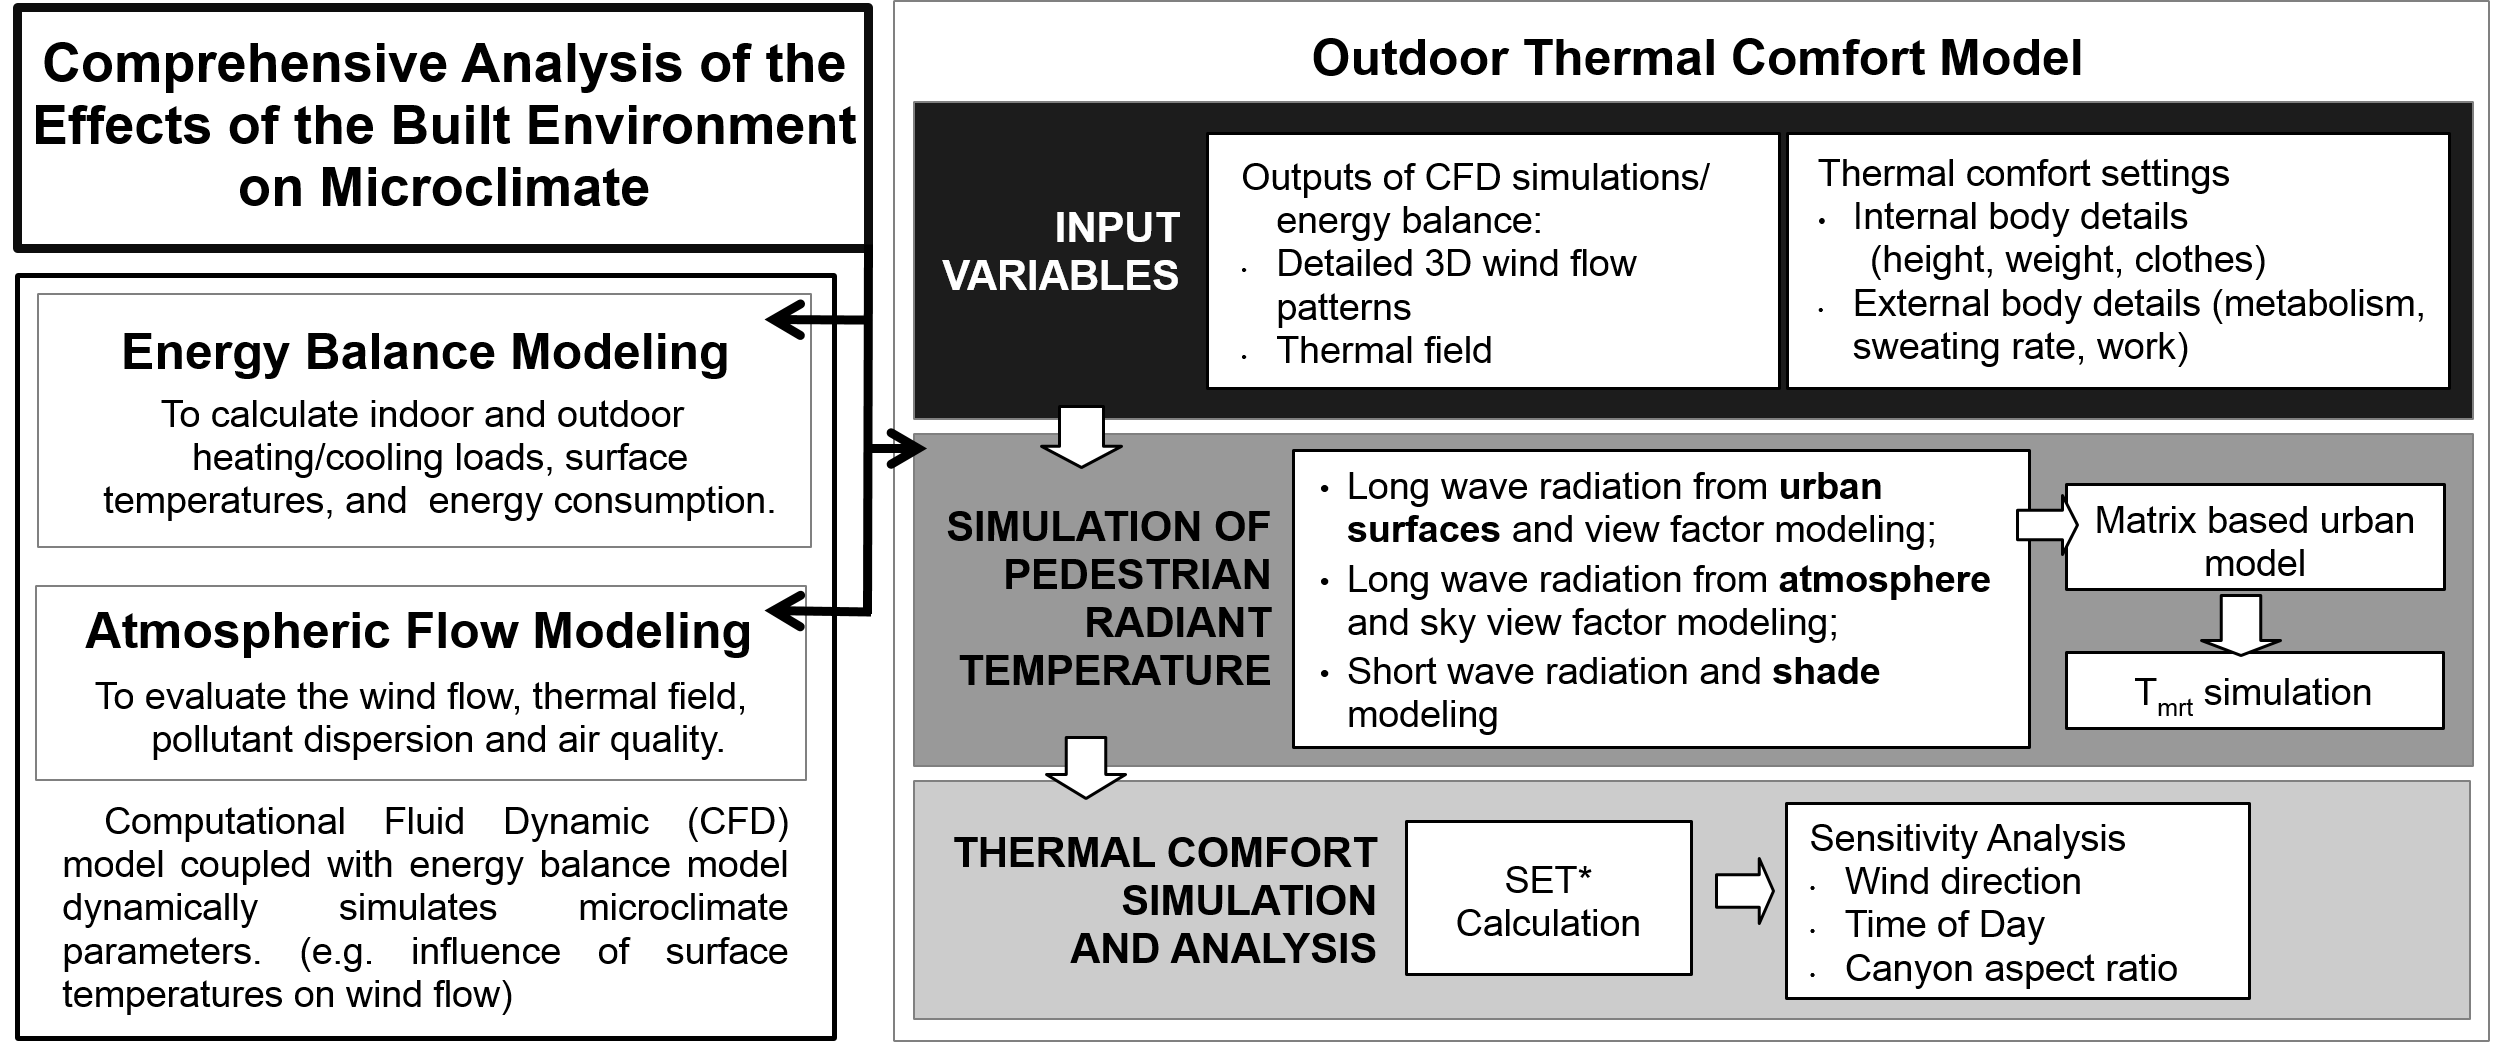
\includegraphics[width=16cm]{flowchartBW.PNG}}
\caption{Flow chart of research process}
\label{Fig.Visibility}
\end{figure}




%T_{mrt}=\sqrt[4]{\frac{1}{\sigma}(a_{p}{\cdot}E_{sol}{\cdot}F_{sol\rightarrow{p}}+\varepsilon_{sky}{\cdot}E_{sky}{\cdot}F_{sky\rightarrow{p}}+\varepsilon{\cdot}E_{urb}{\cdot}F_{urb\rightarrow{p}})}

%margin{how is urban modeling different from CFD modeling?}

%\nomenclature[A]{$s$}{Area of each mesh, m^2}%
\nomenclature[R]{$t$}{Temperature of each of corresponding mesh ($\rm K$)}%
\nomenclature[A]{$SET$}{Standard effective temperature ($\rm K$)}%
\nomenclature[R]{$H_{sk}$}{Heat loss from the skin ($\rm W\, m^{-2}$)}%
\nomenclature[R]{$h_sp$}{Standard heat transfer coefficient ($\rm W\, m^{-2}\,K^{-1}$)}
\nomenclature[R]{$t_{so}$}{Standard operative temperature ($\rm K$)}%
\nomenclature[R]{$w$}{Skin wetness}%
\nomenclature[R]{$h_{es}$}{Standard evaporative heat transfer coefficient ($\rm W\, m^{-2}\,K^{-1}$)}%
\nomenclature[R]{$p_{ssk}$}{Water vapor pressure at skin temperature ($\rm kPa$)}%
\nomenclature[R]{$p_{SET}$}{Saturated water vapor pressure at standard effective temperature ($\rm kPa$)}%

\nomenclature[R]{$T_{mrt}$}{Mean radiant temperature ($\rm K$)}%
\nomenclature[G]{$\sigma$}{Stefan-Boltzmann constant ($\rm 5.67\times10^{-8}\, W m^{-2} K^{-4}$)}%
\nomenclature[R]{$a_{p}$}{Absorption coefficient of solar radiation for a person }%

\nomenclature[R]{$E_{sol}$}{Solar radiation intensity ($\rm W\, m^{-2}$)}%
\nomenclature[R]{$F_{sol-p}$}{View factor between the short-wave sources and a person}%
\nomenclature[G]{$\varepsilon_{sky}$}{Emissivity of the sky }%
\nomenclature[R]{$E_{sky}$}{Long-wave radiation intensity from the atmosphere ($\rm W\, m^{-2}$)}%
\nomenclature[R]{$F_{sky-p}$}{View factor between the visible sky and a person}%
\nomenclature[R]{$E_{urb}$}{Long-wave radiation intensity of urban surfaces ($\rm W\, m^{-2}$)}%
\nomenclature[G]{$\varepsilon_{urb}$}{Emissivity of urban surfaces  }%
\nomenclature[R]{$F_{urb-p}$}{View factor between urban surfaces and a person }%   

%\nomenclature[A]{$A_D$}{Dubois surface area, $m^2$}%
%\nomenclature[A]{$m$}{Body weight, kg}%
%\nomenclature[A]{$l$}{Body height, m}%
%\nomenclature[A]{$q_{sk}$}{total rate of heat loss from skin, $W/m^2$}%
%\nomenclature[A]{$q_{res}$}{total rate of heat loss through respiration, $W/m^2$}%
%\nomenclature[A]{$C_{res}$}{Rate of evaporative heat loss,$W/m^2$}%
%\nomenclature[A]{$E_{res}$}{Rate of evaporative heat loss from respiration, $W/m^2$}%
%\nomenclature[A]{$S_{cr}$}{Rate of heat storage in core compartment, $W/m^2$}%
%\nomenclature[A]{$S_{sk}$}{Rate of heat storage in skin compartment,$W/m^2$}%
%\nomenclature[A]{$C$}{Sum of the convection heat transfer at the outer clothing surface, $W/m^2$}%
%\nomenclature[A]{$R$}{Sum of the radiation heat transfer at the outer clothing surface, $W/m^2$}%
%\nomenclature[A]{$h_r$}{Radiative heat transfer coefficient, $W/m^2K$)}%
%\nomenclature[A]{$h_p$}{Sensible heat transfer coefficient, $W/m^2K$}%
%\nomenclature[A]{$A_r$}{Effective radiation area of body, $m^2$}%
%\nomenclature[A]{$h_{cc}$}{Corrected convective heat transfer coefficient, $W/m^2K$}%
%\nomenclature[A]{$p_t$}{Local atmosphere pressure, kPa}%
%\nomenclature[A]{$T_N$}{Temperature of surface N, K}%
%\nomenclature[A]{$F_{P-N}$}{Angle factor between a person and surface N}%
%\nomenclature[A]{$t_a$}{Air temperature, K}%
%\nomenclature[A]{$w$}{Fraction of wetted skin surface, dimensionless}%
%\nomenclature[A]{$t_{sk}$}{Skin temperature, K}%
%\nomenclature[A]{$p_{sk}$}{Water vapor pressure at skin temperature $t_{sk}$, kPa}%
%\nomenclature[A]{$p_a$}{Water vapor pressure in ambient air, kPa}%
%\nomenclature[A]{$f_{cl}$}{Clothing area factor, dimensionless}%
%\nomenclature[A]{$t_g$}{Ground temperature, K}%
%\nomenclature[A]{$t_w$}{Wall temperature, K}%
%\nomenclature[A]{$A_{cl}$}{Actual surface area of the clothed body, $m^2$}%
%\nomenclature[A]{$I_{cl}$}{Insulation of an ensemble, $(m^2K)/W$}%
%\nomenclature[A]{$M$}{Metabolic Activity, $W/m^2$}%
%\nomenclature[A]{$W$}{Work, $W/m^2$}%
%\nomenclature[A]{$t_{cl}$}{Clothes Temperature, K}%
%\nomenclature[A]{$h_c$}{Convective heat transfer coefficient, $W/(m^2K)$}%
%\nomenclature[A]{$h_{sc}$}{Corrected convective heat transfer coefficient, $W/(m^2K)$}%
%\nomenclature[A]{$LR$}{Lewis ratio, $K/kPa$}%
%\nomenclature[A]{$h_e$}{Evaporative heat transfer coefficient, $W/(m^2K)$}%
%\nomenclature[A]{$h_{ec}$}{Corrective evaporative heat transfer coefficient, $W/(m^2K)$}%
%%\nomenclature[A]{$E_{sk}$}{Total rate of evaporative heat loss from skin, $W m^{-2}$}%
%\nomenclature[A]{$R_{cl}$}{Evaporative heat transfer resistance of clothing area, $(m^2K)/W$}%
%\nomenclature[A]{$W_{rsw}$}{Skin wetness with no regulatory, dimensionless}%
%\nomenclature[A]{$E_{rsw}$}{Evaporative heat loss by regulatory sweating, $(m^2K)/W$}%
%\nomenclature[A]{$E_{max}$}{Maximum possible evaporative heat loss, $(m^2K)/W$}%
%\nomenclature[A]{$\dot{m}_{rsw}$}{Rate at which regulatory sweat is generated, $kg/(sm^2)$}%
%\nomenclature[A]{$h_{fg}$}{Heat of vaporization of water, $J/kg$}%
%\nomenclature[A]{$I$}{Intrinsic insulation of air layer, $m^2K/W$}%
%\nomenclature[A]{$S_{str}$}{Mean radiant flux density, $W/m^2$}%
%\nomenclature[A]{$\varepsilon_{p}$}{Emissivity of the human body}%
%\nomenclature[A]{$L_i$}{Long wave radiant fluxes of surface i, $W/m^2$}%
\nomenclature[R]{$P$}{Water vapor pressure ($\rm kPa$)}%
%\nomenclature[A]{$P_{so}$}{Uniform water vapor pressure, kPa}%
%\nomenclature[A]{$h$}{Sum of radiative and convective heat transfer coefficient, $W m^{-2}$}%
%\nomenclature[A]{$t_o$}{Operative temperature, $W/m^2$}%
\nomenclature[R]{$h_{sp}$}{Standard heat transfer coefficient ($\rm W\, m^{-2}$)}%
\nomenclature[R]{$SR$}{Total irradiance  ($\rm W\, m^{-2}$)}%
%\nomenclature[A]{$E_{dir}$}{Direct irradiance, $W/m^2$}%
%\nomenclature[A]{$WBGT$}{Wet bulb globe temperature, K}%
%\nomenclature[A]{$NWB$}{Natural wet bulb temperature, K}%
%\nomenclature[A]{$GT$}{Globe temperature, K}%
%\nomenclature[A]{$T_{rso}$}{Mean radiant temperature effected by solar radiant, K}%
\nomenclature[R]{$v$}{Wind velocity  ($\rm m \, s^{-1})$}%
%\nomenclature[A]{$D$}{Globe diameter, m}%
%\nomenclature[A]{$T_{rsu}$}{Mean Radiant temperature effected by urban ground and walls, K}%
%\nomenclature[A]{$F_{dA-P}$}{Angle factor between the mesh and the person}%
%\nomenclature[A]{$A_p$}{projected area on a plane perpendicular to the direction to the mesh}%
%\nomenclature[A]{$A_{eff}$}{effective radiation area of the person}%



\begin{table*}[!t]
  \begin{framed}
  \footnotesize
    \printnomenclature
  \end{framed}
\end{table*}

%%%%%%%%%%%%%%%%%%%%%%%%%%%%%%%%%%%%%%%%%%%%%%%%%%%%%%%%%%%%%%%%%%%%%%%%%%%%%%%%%%%%%%%%%%%%%%%%%%%%%

\section{Methods}
\subsection{Gridded Urban Model}
The geometry of the idealized model consists of a 3x3 matrix of equally spaced cubic buildings (\ref{Fig.IdealUrban}). The SET calculation occurs on a mesh grid over the urban model, wherein individual parameters are stored and analyzed  (Fig. \ref{Fig.GroundMesh}). This allows for detailed analysis of spatial variation in thermal comfort. SET is calculated for a pedestrian standing at every grid point along the model.

\begin {figure}[h]
\graphicspath{ {image/} }
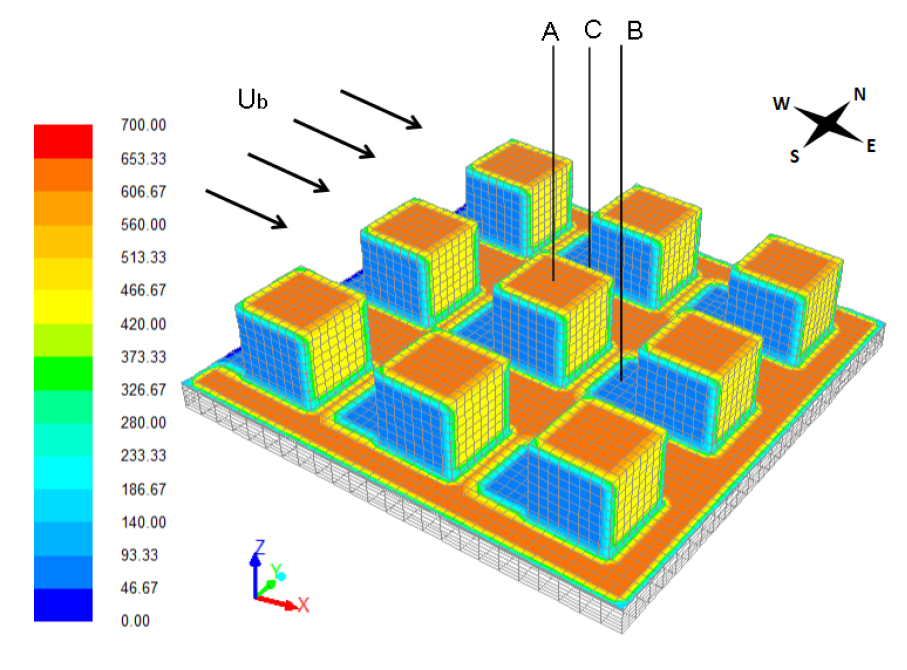
\includegraphics[width=7cm]{ThermalEnvironmentModel.PNG}
\centering
\caption{Idealized configuration of the urban environment for CFD modelling \cite{nazarian2014effects}}
\label{Fig.IdealUrban}
\end {figure}

%\begin{figure}[H]
%\graphicspath{ {image/} }
%\centering
%\subfigure[Cross-section of the urban model mesh]{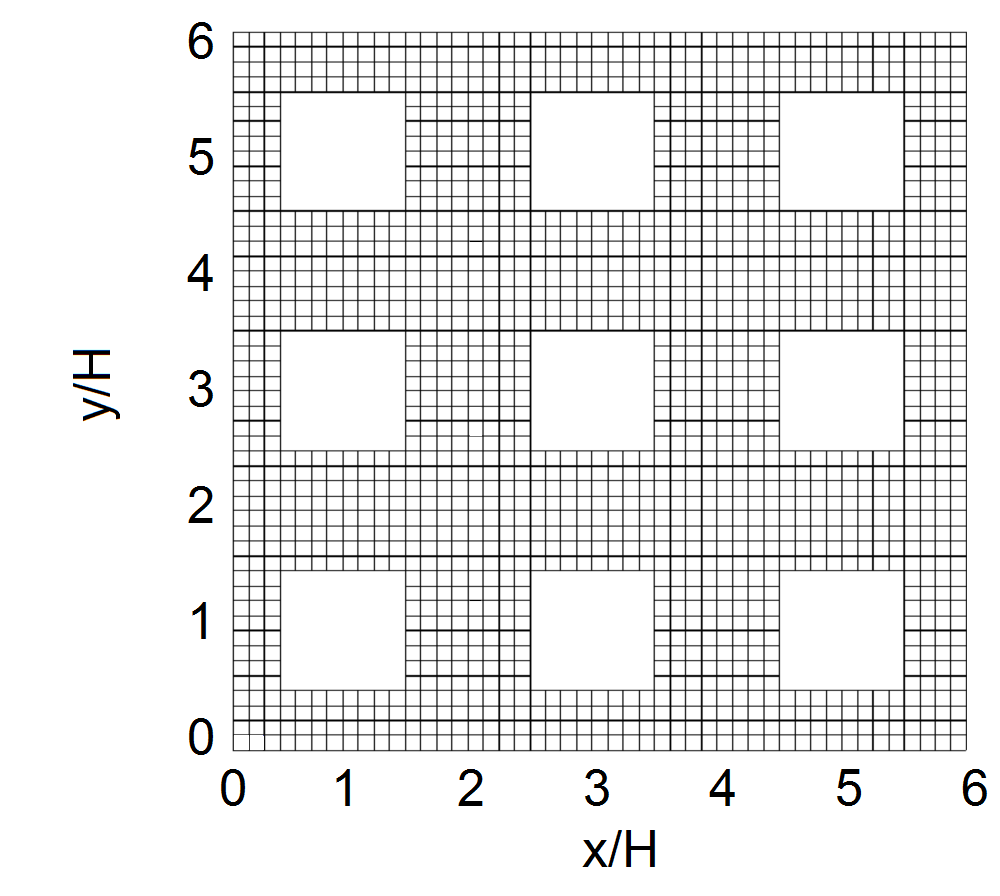
\includegraphics[width=2in]{groundold.png} }
%\hskip 0.4in 
%\centering
%\subfigure[Distribution of the air temperature at the pedestrian level (z=1.5 m) input from the CFD simulation at 1200 PST \cite{nazarian2014effects, nazarian2015cfd}]{
%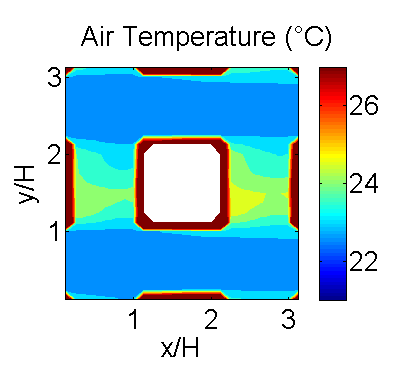
\includegraphics[width=2.2in]{AirTemp_BaseCase.png}}
%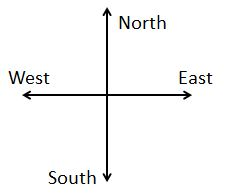
\includegraphics[width=1in]{ESWN.JPG}
%\caption{Parameters, such as temperature, are analyzed point by point throughout the mesh representing the urban model.}
%\label{Fig.GroundMesh}
%\end{figure}

\subsection{CFD Simulation Input}
In a previous study by Nazarian and Kleissl \cite{nazarian2014effects, nazarian2015cfd}, the urban microclimate for an 3-D idealized configuration of a compact mid-rise urban environment was simulated using a Computational Fluid Dynamic (CFD) model. The CFD software tool ANSYS FLUENT 14.5 was used to simulate flow field and heat transfer in a 3D idealized configuration. Meteorological data from a representative coastal urban weather station in southern California (San Diego, 32.867 N, 117.133 W) on a clear summer day was used. As shown in Fig. \ref{Fig.IdealUrban}, the flow passes over a matrix of 3x3 evenly spaced buildings with a ground surface albedo of 0.18. Periodic boundary conditions are used such that the 3x3 configuration represents a unit cell within an infinite array of uniformly spaced buildings. Shortwave and longwave radiation are calculated at each time step and the flow field is dynamically coupled with the thermal field. The walls of the model do not include windows and latent heat flux is neglected. The simulation results were validated against field measurements and compared to other energy balance models. Refer to \cite{nazarian2014effects, nazarian2015cfd} for more information on the simulation setup and configuration.

% While these simulations provide detailed information on the urban climate, they are not sufficient for understanding thermal comfort. Human sensation of the thermal environment is affected by the combined and counteracting effects of several parameters, including wind, temperature, and radiant heat transfer from the human body, that are not taken into account in the CFD model.\jan{Most readers would understand this.} 

\vspace{3ex}

\subsection{Calculation of Standard Effective Temperature}
Standard effective temperature (SET) was the index chosen to quantify and analyze thermal comfort. The standard effective temperature (SET) is defined as the equivalent temperature of an isothermal environment at 50 percent relative humidity at which a subject, while wearing typical clothing, would have the same heat stress (skin temperature, $T_sk$ ) and thermoregulatory strain (skin wetness, w) as in the actual test environment. Based on the dynamic Pierce two-node model of human temperature regulation, SET accounts for both body skin and body core. The body core node represents the metabolic system and heat exchange inside the body, and the body skin node represents skin, perspiration system, clothes and external heat exchange. The equation for SET can be expressed as \cite{gagge1986standard}

\begin{equation}
H_{sk}=h_{sp}(t_{so}-SET)+wh_{es}(P_{ssk}-0.5P_{SET}),
\label{Eqa.SET}
\end{equation}

where $H_{sk}$ ($\rm W\, m^{-2}$) is the heat loss from skin; $h_{sp}$ ($\rm W\, m^{-2}\,K^{-1}$) is the standard heat transfer coefficient; $t_{so}$ ($K$) is the standard operative temperature; $w$ (-) is the fraction of the wetted skin surface; $h_{es}$ ($\rm W\, m^{-2}\,K^{-1}$) is the standard evaporative heat transfer coefficient; $P_{ssk}$ ($\rm kPa$) is the water vapor pressure at skin, assumed to be that of saturated water vapor at skin temperature; and $P_{SET}$ ($\rm kPa$) is the saturated water vapor pressure at SET. In this study, SET ($^{\circ}$C) is analyzed at steady state, i.e. without change in heat storage within the body. Therefore, $H_{sk}$ is assumed to be zero. The accuracy of SET calculations are improved by modelling mean radiant temperature, which contributes to $t_{so}$, the standard operative temperature. \jan{Call out more explicitly what the relationship between t_o and MRT is.}

\subsection{Mean Radiant Temperature Modeling}
The effect of radiation on the thermal sensation is represented by mean radiation temperature ($T_{mrt}$), which is the uniform temperature of an imaginary enclosure in which radiant heat transfer from the human body is equal to those in the actual non-uniform enclosure. $T_{mrt}$ is a key factor in calculating the standard operating temperature ($t_{so}$) and thus is an important variable in human thermal comfort. Outdoor simulations of $T_{mrt}$ are difficult due to complex geometry and solar conditions. Huang et al. \cite{huang2014citycomfort+} introduces a method to simulate the spatial variation of $T_{mrt}$. He derives $T_{mrt}$ by modeling three primary components of radiation fluxes: shortwave radiation (diffuse, direct and reflected), atmospheric longwave radiation and longwave radiation from urban surfaces. Each component is weighted by their view factors relative to the position of the pedestrian.
\begin{equation}
T_{mrt}=\sqrt[4]{\frac{1}{\sigma}(a_{p}{\cdot}E_{sol}{\cdot}F_{sol\rightarrow{p}}+\varepsilon_{sky}{\cdot}E_{sky}{\cdot}F_{sky\rightarrow{p}}+\varepsilon{\cdot}E_{urb}{\cdot}F_{urb\rightarrow{p}})}
\label{Equ.MRT}
\end{equation}
The first term denotes the shortwave radiation from sun, i.e. direct solar radiation. The second term is the atmospheric longwave radiation, and the third term is the longwave radiation from urban surfaces. Huang et al. has verified the accuracy of this method in the same paper\cite{huang2014citycomfort+}. However, in order to simplify the simulation, shading effects are ignored and the sky view factor, $F_{sky\rightarrow{p}}$, is assumed to be constant. Thus, to further improve spatial accuracy, this method is developed by adding shade and sky view factor modeling.

\subsubsection{Shortwave radiation and shade modeling}
Shortwave radiation denotes the sum of intensity of direct, diffuse, and reflected solar radiation. Solar radiation components are output by ANSYS Fluent's solar ray-tracing algorithm and further analyzed. Since diffuse radiation is often considered to be uniform in computational simulations \cite{flint1998solar, sreekumar1998egret, madronich1999role}\jan{Uniform and isotropic are two different things. Make sure you use them correctly.}, and reflected radiation is only a small proportion of the total radiation (fig. \ref{Fig.SolarIntensity}), this paper considers both diffuse and reflected radiation as isotropic. 

\begin{figure}[H]
\graphicspath{ {image/} }
\centerline{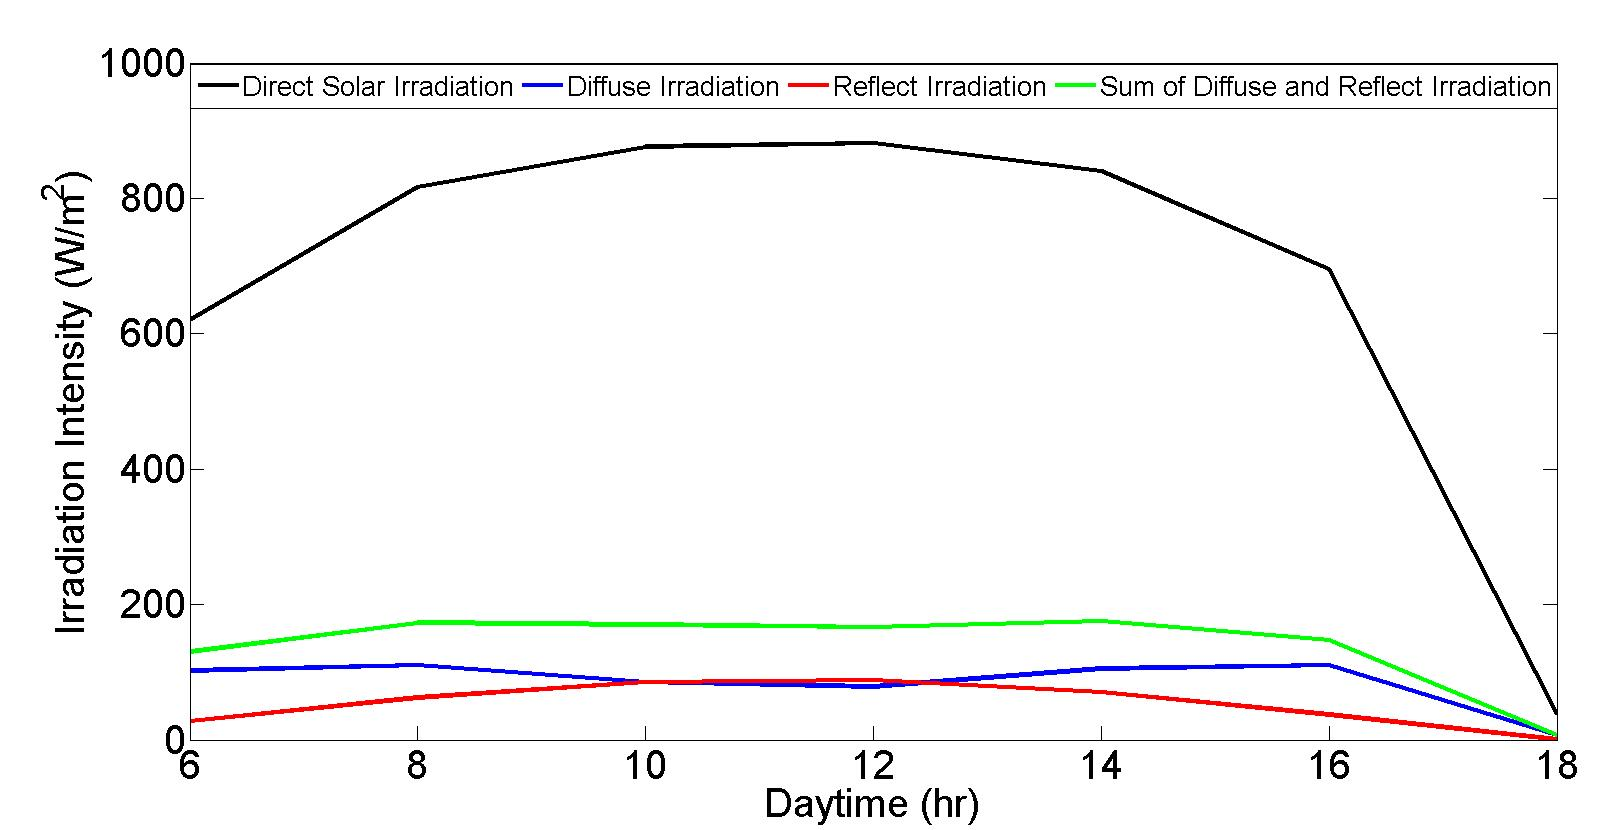
\includegraphics[width=14cm]{SolarIntensity.jpg}}
\caption{Solar intensity throughout the day at the pedestrian level.\jan{Averaged over the domain?}}
\label{Fig.SolarIntensity}
\end{figure}

Conversely, on the clear day simulated, direct solar radiation is the most dominant component. It represents solar radiation traveling directly to the surface of the earth, and is non-zero only in unshaded areas. It is therefore important to isolate sunlit areas by accounting for shade. Several geometrical relations for the urban model are developed in order to outline shaded areas according to solar position (Fig. \ref{Fig.Shadow}). 
\begin{figure}[H]
\graphicspath{ {image/} }
\centerline{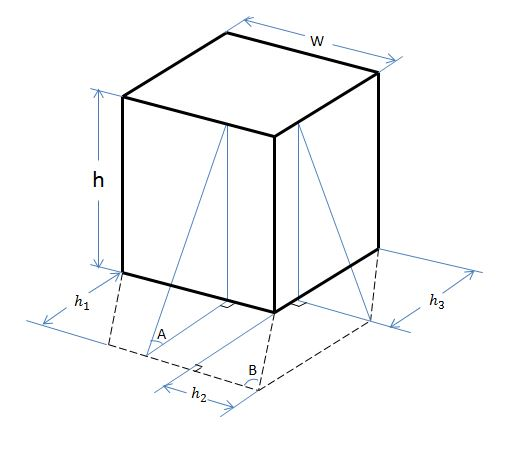
\includegraphics[width=10cm]{SVFModel.JPG}}
\caption{Shadow model description (Dashed lines indicate edges of shaded area)}
\label{Fig.Shadow}
\end{figure}


\begin{equation}
\centering
\begin{split}
A=&atan(\frac{x}{y})\\
h_1=&\frac{h}{tan(A)}\\
B=&atan(\frac{y}{z})\\
h_2=&\frac{H_1}{tan(B)}\\
h_3=&\frac{H_2}{tan(90-B)}\\
\end{split}
\end{equation}
\noindent where $x,y,z$ are vector components to the sun. $A, B, h_1, h_2, h_3$ are applied to the side(s) of the building that are not facing the sun.

These geometric calculations of shading effects provide an accurate direct solar radiation field. For example, in the shade model of the urban area at 1000 PST, shade accumulates at the west side of the buildings and also covers a smaller area to the north of the building, as shown in Figure \ref{Fig.ShadowExample}.  

\begin{figure}[H]
\graphicspath{ {image/} }
\centering
\vcenter{\hbox{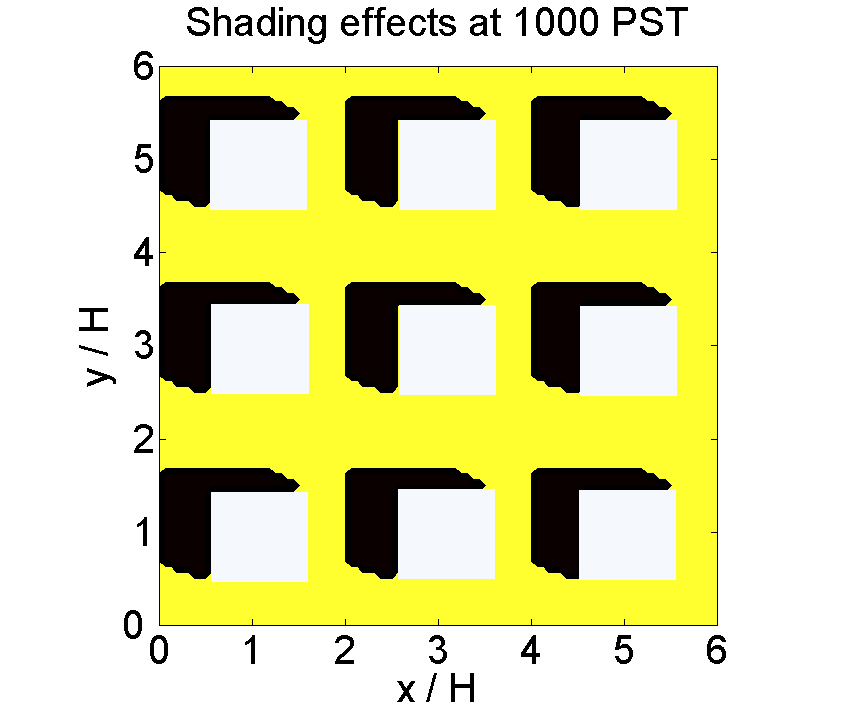
\includegraphics[width=8cm]{ShadowSample.png}}}
\vcenter{\hbox{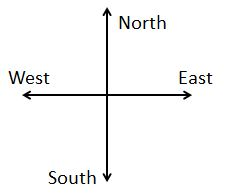
\includegraphics[width=1in]{ESWN.JPG}}}
\caption{Example of building shade model at 1000 PST (black indicates shaded area; yellow is sunlit area)}
\label{Fig.ShadowExample}
\end{figure}


\subsubsection{Longwave radiation from the atmosphere and view factor modeling}
In addition to shortwave radiation, mean radiant temperature also depends on sky longwave radiation, which describes the longwave radiation received from the atmosphere. To improve the accuracy of Huang's $T_{mrt}$ model, longwave radiation from the sky needs to be weighted by the sky view factor (SVF). SVF is calculated as the fraction of area covered by sky when viewed from the ground up. Wu \cite{wu2013calculation} introduces a simplified estimation method of SVF in urban areas without sacrificing spatial accuracy. Wu’s method derives SVF from the wall view factors (WVF) calculated using the azimuth ($\gamma$) and altitude ($\beta$) angles to the building.

\begin{equation}
\rm
WVF_{M2}=\frac{1}{2\pi}
\left\{
(\gamma_2-\gamma_1)+cos{\beta}[tan^{-1}(cos{\beta}tan{\gamma_1})-tan^{-1}(cos{\beta}tan\gamma_2)]
\right\}
\end{equation}
\begin{equation}
\rm SVF_{ref-M2}=1-(\rm WVF_{1-M1}+\rm WVF_{2-M2})
\end{equation}

where $\rm WVF_{M1}$ and $\rm WVF_{M2}$ indicate wall view factors in two different directions \cite{wu2013calculation}\jan{Define ``different directions.'' Define assumptions in Wu's model. Explain the logic of the notation used here ref-M2, 1-M1 etc.}. An example of SVF modeling is presented in Figure \ref{Fig.SVFexample}. 

\begin{figure}[H]
\graphicspath{ {image/} }
\centerline{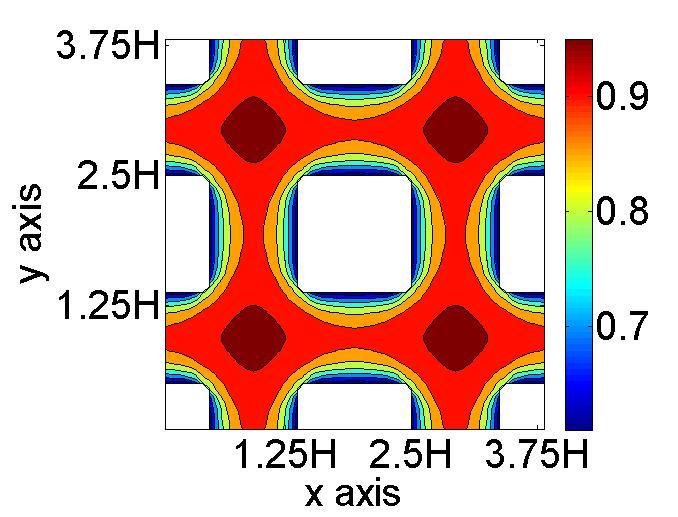
\includegraphics[width=8cm]{SVFSample.jpg}}
\caption{Sky view factor (color bar) in the center of the domain with canyon aspect ratio 1/2 (= canyon height divided by canyon width).}
\label{Fig.SVFexample}
\end{figure}



\subsubsection{Longwave radiation from urban surfaces and urban surface visibility modeling}

The third term of $T_{mrt}$ in Eq. \ref{Equ.MRT} describes longwave radiation received from building and ground surfaces. The temperature of each surface must be weighted by view factors, i.e. the proportion of radiation released from surface A that intercepts the pedestrian. The matrix-based model calculates the view factor between two different points with a simple algorithm.

The algorithm analyzes a line between any pair of urban ground surfaces \jan{any two pixels? For ``surfaces'' there exists partial visibility.} and checks if the line intersects with a building (i.e. whether the radiation between these two points are blocked). A visibility matrix is then generated for each pedestrian location for a point at pedestrian height. 

The figure \ref{Fig.VisibilityExample} show examples of visibility modeling at pedestrian height.\jan{Visibility only defines which surfaces should be included in the MRT calculation. But how is longwave MRT actually calculated? Also state assumptions on periodicity of domain. I assume you are not considering surfaces that cross the simulation domain boundary.}


\begin{figure}[H]
\centering  
\graphicspath{ {image/} }
\subfigure {   
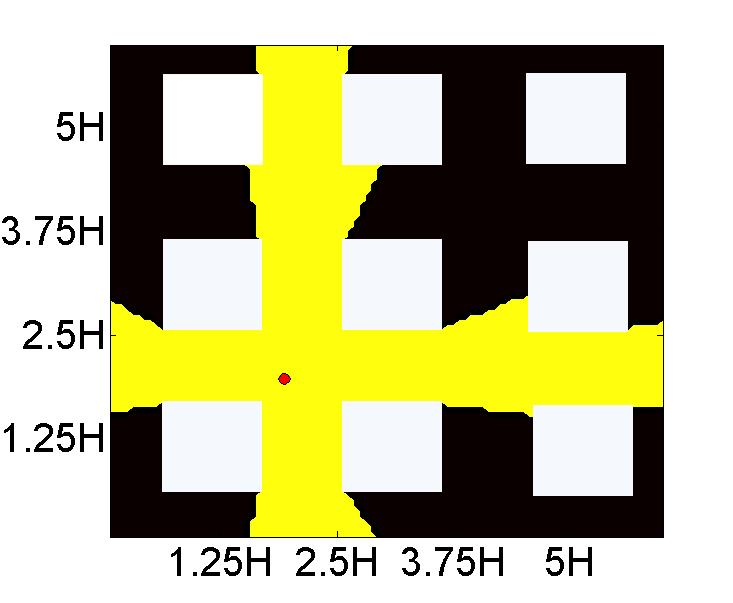
\includegraphics[width=7cm]{VisibilityTestExampleOne.jpg}}    
\subfigure {    
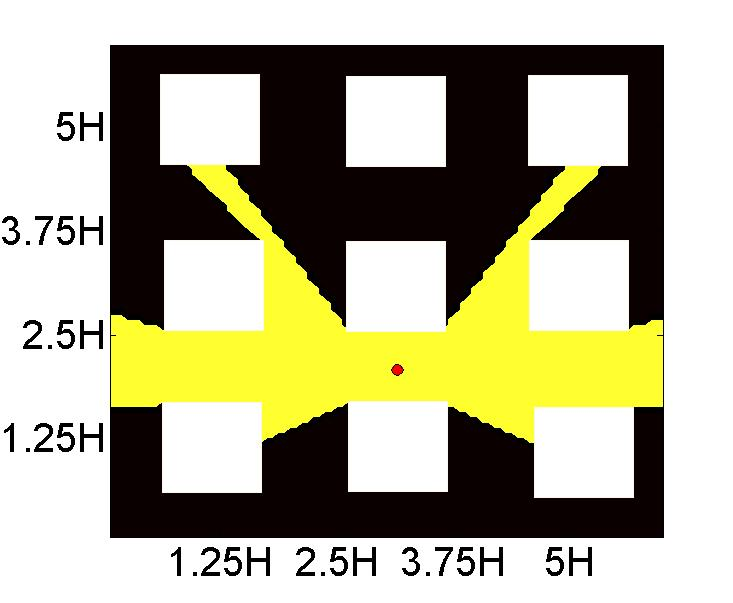
\includegraphics[width=7cm]{VisibilityTestExampleTwo.jpg}}

\caption{Visibility modeling examples in a horizontal plane\jan{What about 3D?}. Red denotes the pedestrian location, yellow denotes visible area, black denotes invisible area, and white denotes building projection. Left: Pedestrian at at (1.875$H$, 1.875$H$). Right: Pedestrian at (1.875$H$, 3.125$H$).}
\label{Fig.VisibilityExample}
\end{figure}



%%%%%%%%%%%%%%%%%%%%%%%%%%%%%%%%%%%%%%%%%%%%%%%%%%%%%%%%%%%%%%%%%%%%%%%%%%%%%%%%%%%%%%%%%%%%%%%%%%%%%
\section{Simulation Results}
\jan{This paragraph belongs in methods section.}}
Thermal comfort is simulated for a man who is 173~cm tall and weighing 70~kg, with typical summer clothes, standing motionless in San Diego, California, USA on a clear summer day. The calculations are made at the pedestrian level of 1.5~m above ground. Average wind velocity is 2~m/s at a height two times that of the building. 

\subsection{Spatial variation of thermal comfort}

Thermal comfort values are represented as SET distributions in a cross-section of the urban model at the pedestrian height (Fig.  \ref{Fig.Parameters}). These results verify that SET is heterogeneous across small urban areas despite small variations in air temperature. In order to better understand the determinants of thermal comfort, the SET distribution is compared to the initial CFD inputs such as air temperature, wind speed, and ground temperature, as well as the calculated MRT. Several other parameters, such as sky view factor and pressure, are not shown but still incorporated into the SET calculation.  

\begin{figure}[H] \centering  
\graphicspath{ {image/} }
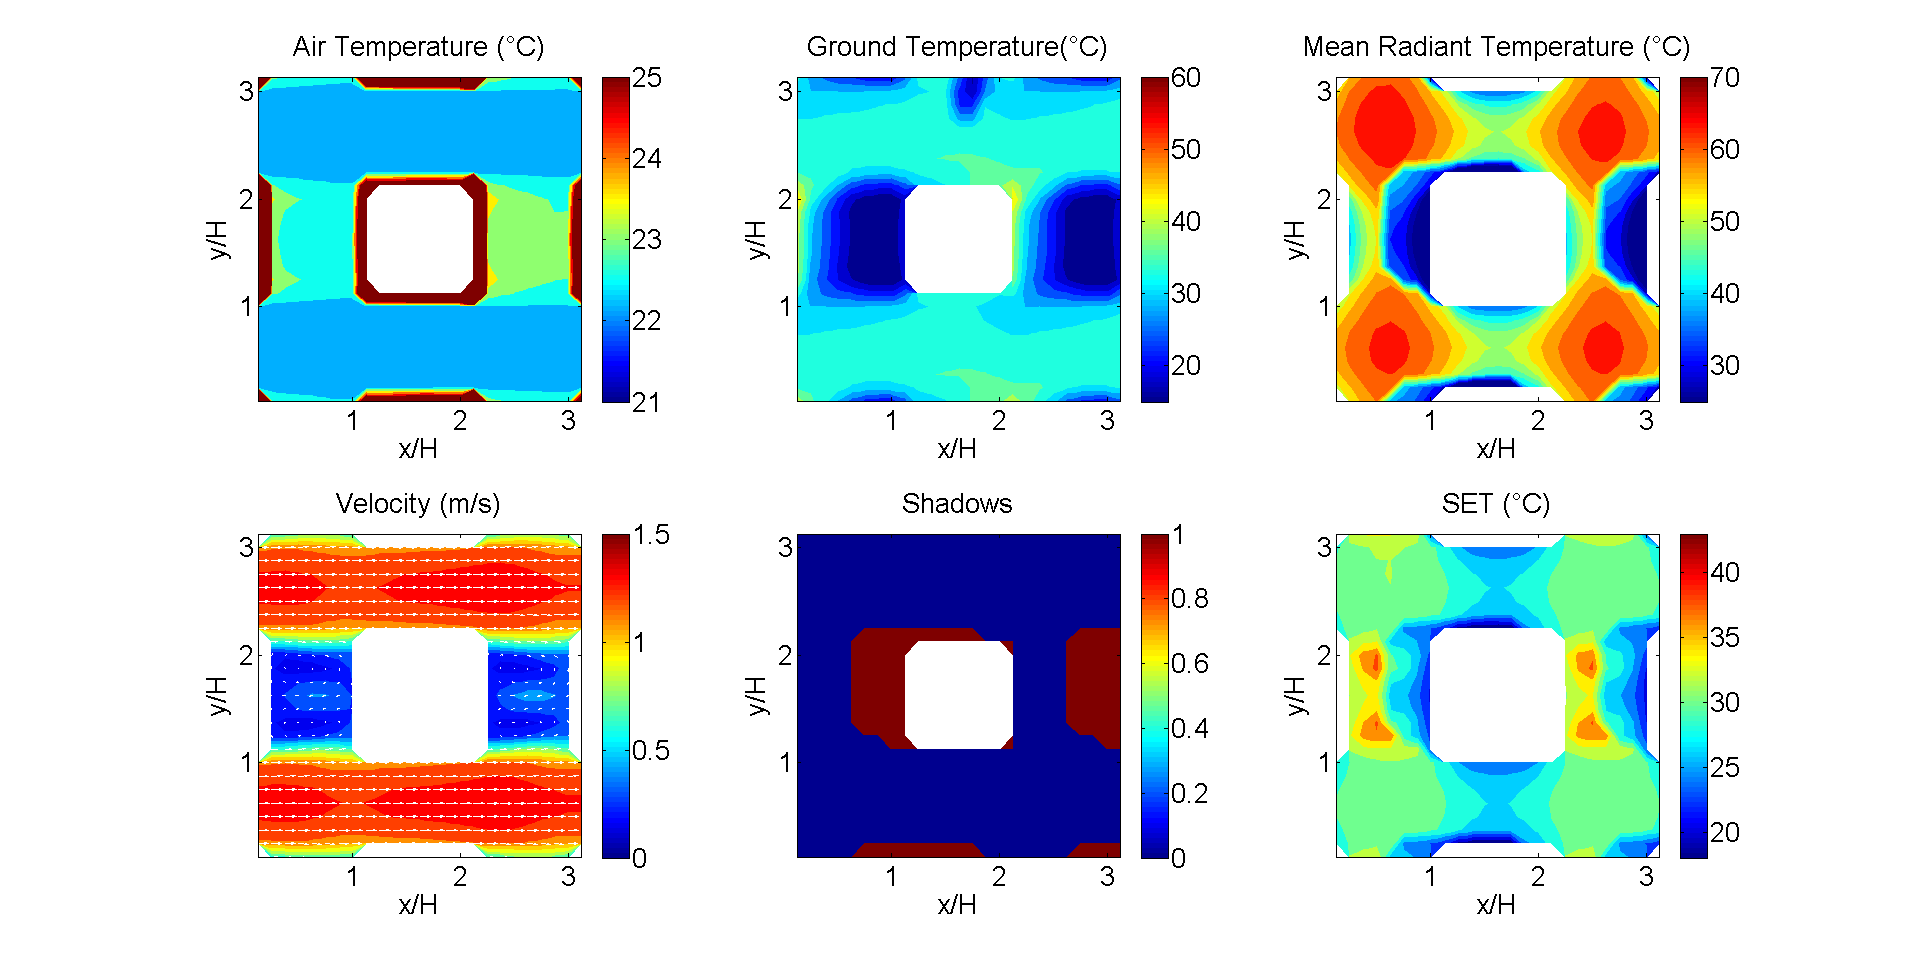
\includegraphics[width=14cm]{1000PST_flux.png}
\hskip 0.5in
\caption{Spatial distribution of different thermal comfort parameters around the center building at 1000~PST} 
\label{Fig.Parameters}
\end{figure}

The aggregate effects of micro-climate in determining thermal comfort are clear. While air temperature remains within 1~K for most of the idealized model, the building wakes with low wind speed significantly increase SET in the span-wise urban canyons compared to the stream-wise urban canyons. \jan{Discuss MRT first which is dominated by incident shortwave.} Meanwhile, the effects of longwave radiation from the ground are most prominent in the shaded areas of the span-wise canyons\jan{I don't see this. I rather think that the peak in SET in the spanwise canyon is driven by direct shortwave combined with large east wall temperature of the adjacent building}. Due to the large ground view factor relative to other sources of radiation, the ground temperature distribution is representative of surface heating from short-wave radiation. 

Spatial variation of thermal comfort is further shown by evaluating the SET distribution along different paths in the street canyons.  The two paths examined are shown in Fig. \ref{Fig.Paths}, and Figs. \ref{Fig.LineSum} and \ref{Fig.LoopSum} show variation of SET along these paths.

\begin{figure}[H] \centering  
\graphicspath{ {image/} }
\subfigure[] { 
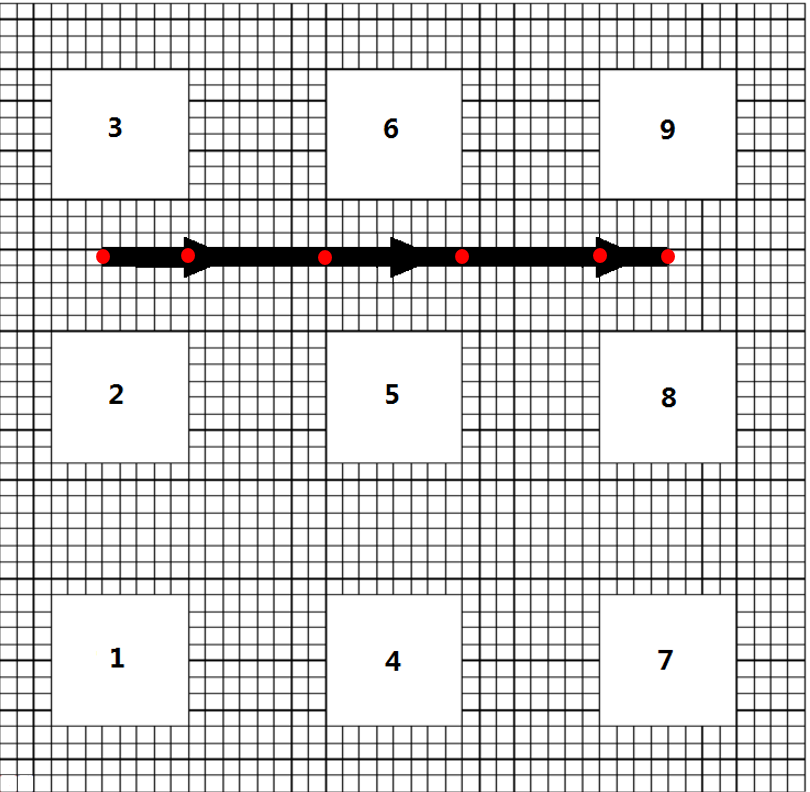
\includegraphics[width=6cm]{LineLocation.png}
\label{Fig.Line}}    
\hskip 0.5in
\subfigure[] { 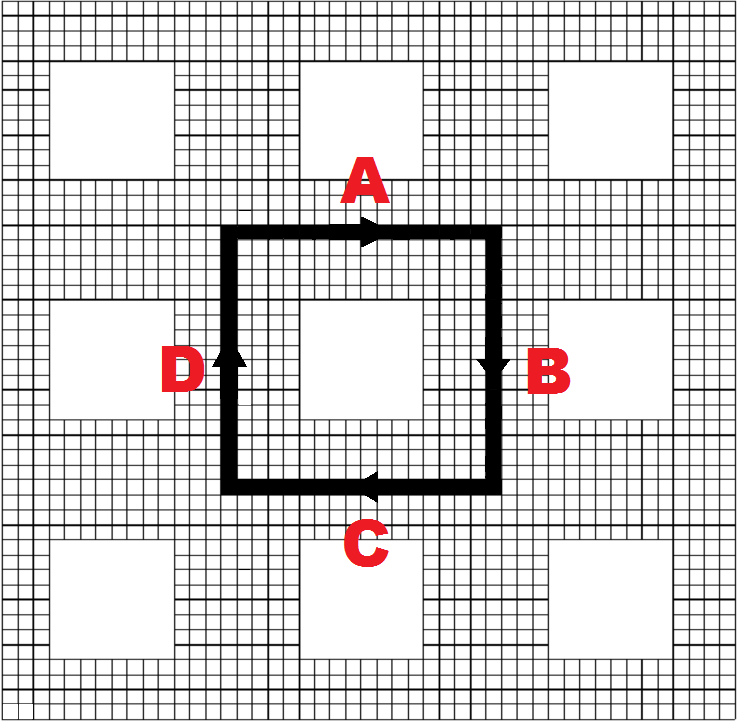
\includegraphics[width=6cm]{CircleLocation.png}\label{Fig.Loop}}
\hskip 0.5in 
\caption{Test set up for SET distributions along a path. Left: Path through a stream-wise urban canyon. Right: Path through the center of the canyon around a building.\jan{Better to integrate these paths in Figs. 5 or 7.}} 
\label{Fig.Paths}
\end{figure}

\begin{figure}[H]
\graphicspath{ {image/} }
\centerline{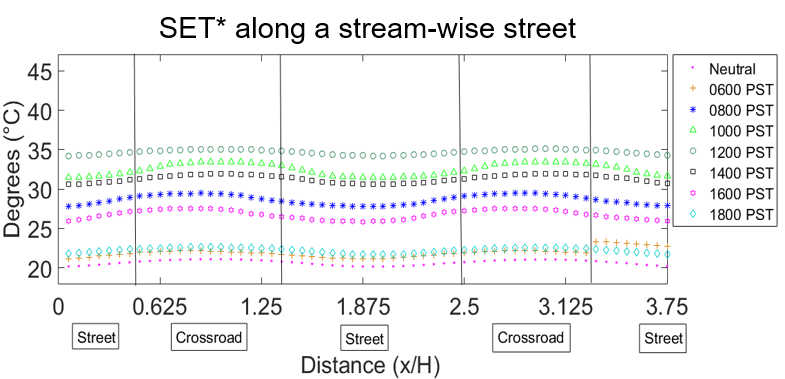
\includegraphics[width=10cm]{line_sum.png}}
\caption{SET distribution at pedestrian height following the path from Fig. \ref{Fig.Line} at different times of day.\jan{This figure is relatively uninteresting.}}
\label{Fig.LineSum}
\end{figure}

\begin{figure}[H]
\graphicspath{ {image/} }
\centerline{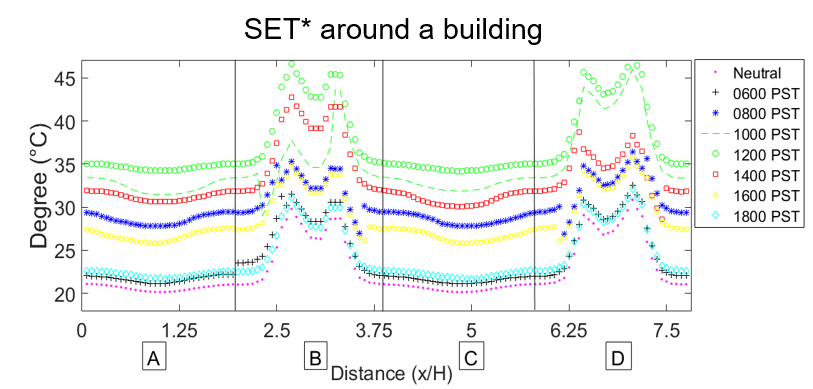
\includegraphics[width=10cm]{loop_sum_final.png}}
\caption{SET distribution on following the path from figure  \ref{Fig.Loop}\jan{Make this Fig. 10b. Showing A and B would be sufficient as C and D should be identical due to symmetry. Remove figure title.}}
\label{Fig.LoopSum}
\end{figure}


The path through the stream-wise canyon (figure \ref{Fig.LineSum}) has significantly smaller variability in SET, with a range of 2.1$^{\circ}$C at 1000~PST, than in the span-wise canyon (figure \ref{Fig.LoopSum}) which has a 14.6$^{\circ}$C SET range. The comparison between streets parallel and perpendicular to the wind flow shows that effects of wind patterns on SET are significant, since SET values increase by about 5~K in the building wake. 

The neutral SET calculation refers to the model with uniform surface temperatures, which excludes shortwave radiation, representing only the effects of wind and longwave radiation. Thus, as shown in the stream-wise path, wind patterns do create differences between crossroads and street areas, but these fluctuations are magnified when combined with the effects of shortwave radiation. 




\subsection{Daily variation of thermal comfort and shade effect}

Thermal comfort is calculated and represented as spatial distributions of SET values in Table \ref{table:DiurnalDist}. We observe the changes in the SET distribution throughout the day from 0600 to 1800 PST in two hour intervals, and compare it to neutral conditions (where surface temperatures are constant) and ground temperature distributions. 

\begin{table}[]
\centering
\caption{Diurnal variation in ground temperature and SET distributions.}
\label{table:DiurnalDist}
\begin{tabular}{cccll}
\cline{1-3}
\multicolumn{1}{|c|}{Neutral Case} & \multicolumn{1}{c|}{0600 PST} & \multicolumn{1}{c|}{1000 PST} &  &  \\ \cline{1-3}
\multicolumn{1}{|c|}{\graphicspath{{image/}}
\raisebox{-\totalheight}{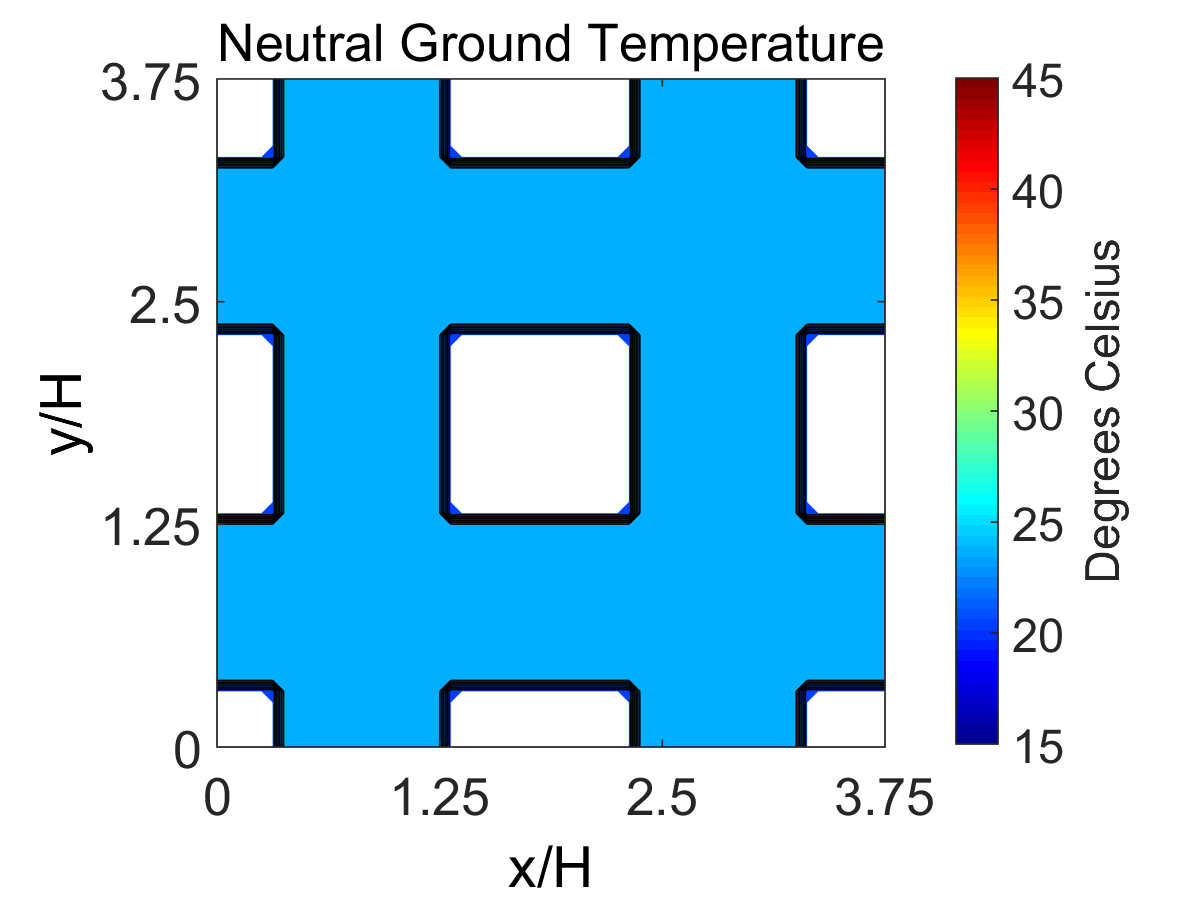
\includegraphics[width=5cm]{GroundN.png}}} & 
\multicolumn{1}{c|}{\graphicspath{{image/}}\raisebox{-\totalheight}{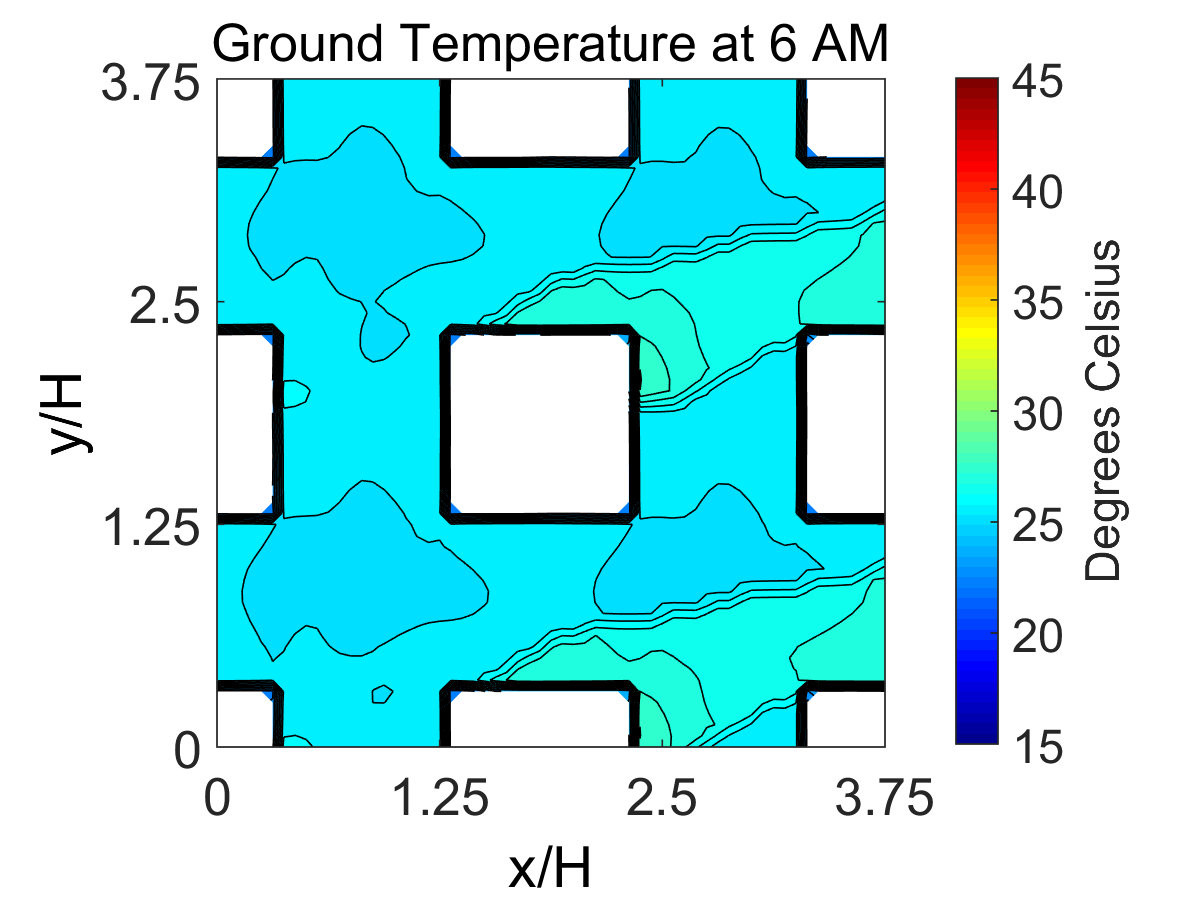
\includegraphics[width=5cm]{Ground6AM.png}}} & 
\multicolumn{1}{c|}{\graphicspath{{image/}}\raisebox{-\totalheight}{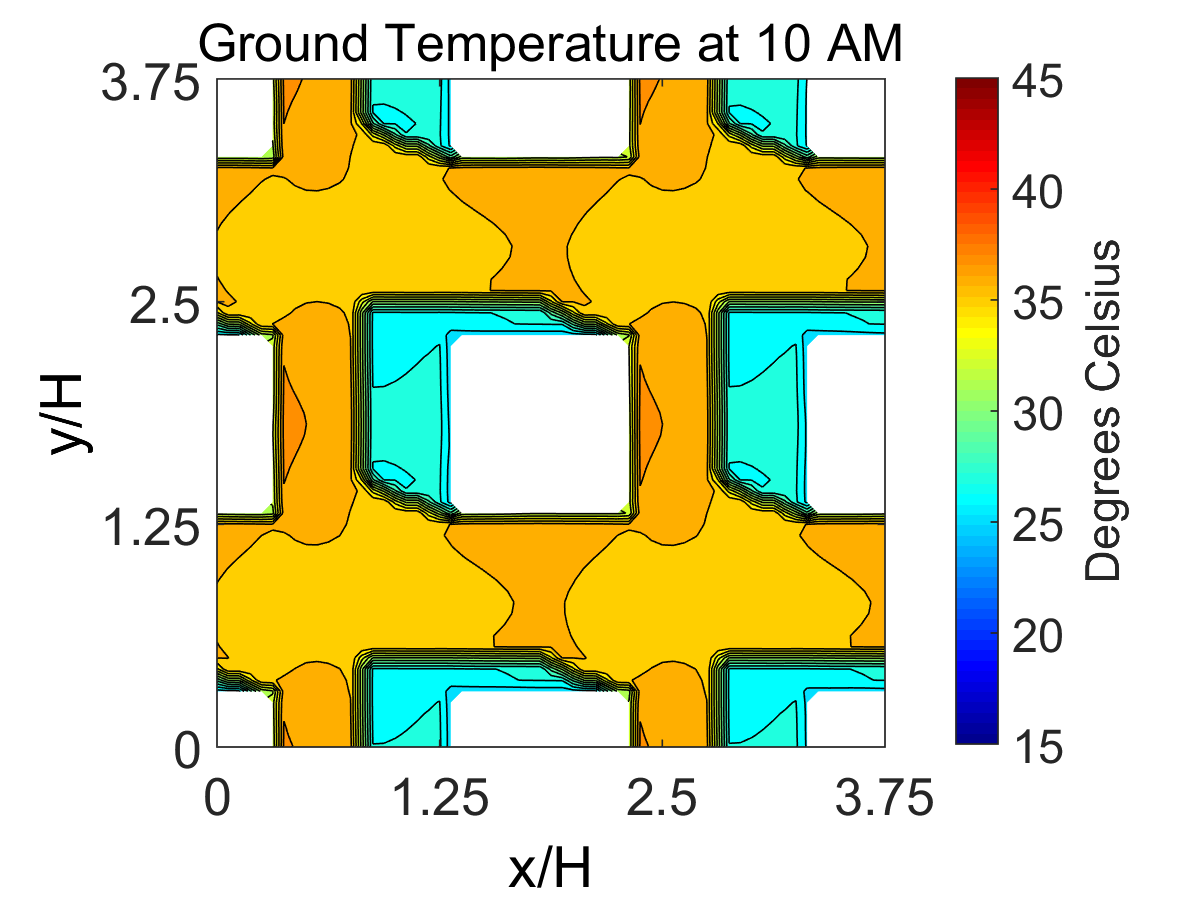
\includegraphics[width=5cm]{Ground10AM.png}}}
&  &  \\ \cline{1-3}
\multicolumn{1}{|c|}{\graphicspath{{image/}}\raisebox{-\totalheight}{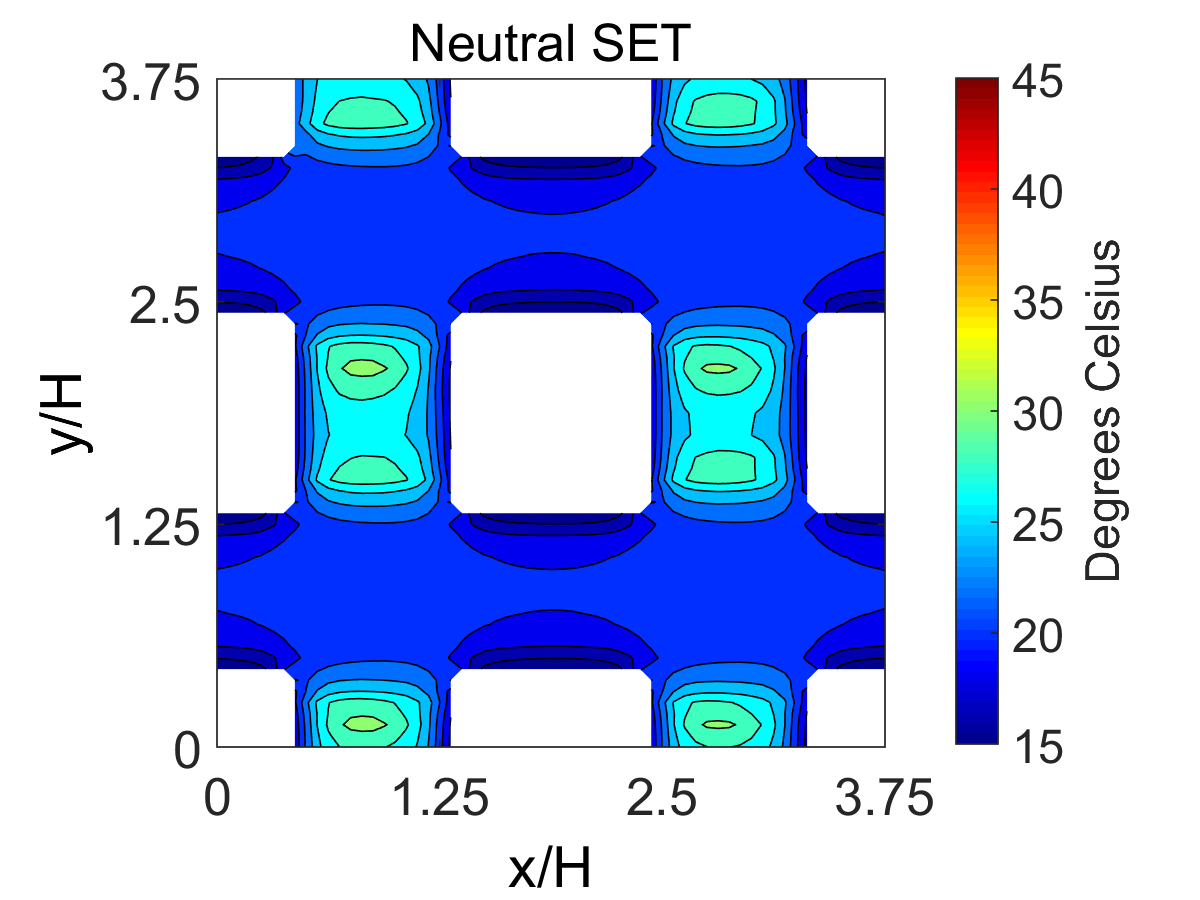
\includegraphics[width=5cm]{SETNeutral.png}}} & 
\multicolumn{1}{c|}{\graphicspath{{image/}}\raisebox{-\totalheight}{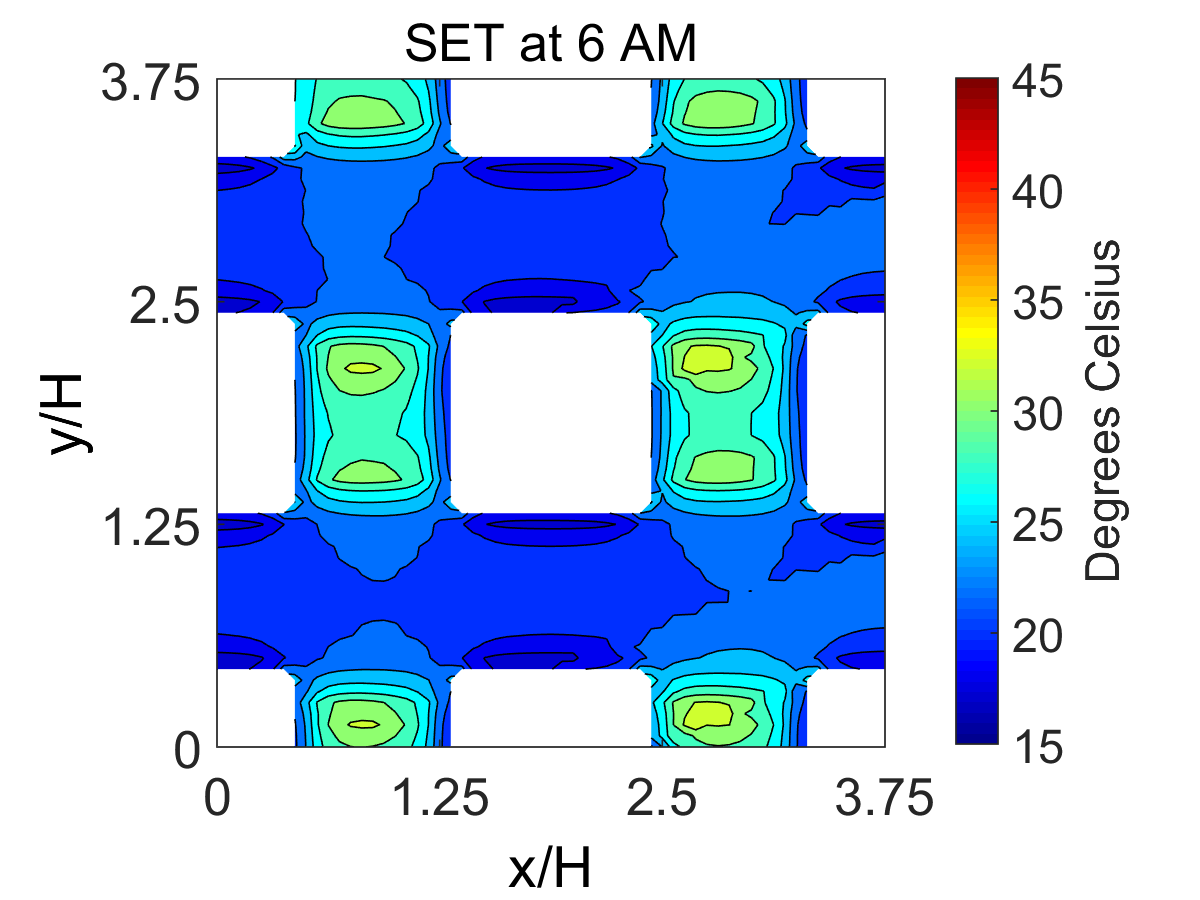
\includegraphics[width=5cm]{SET6AM.png}}} & 
\multicolumn{1}{c|}{\graphicspath{{image/}}\raisebox{-\totalheight}{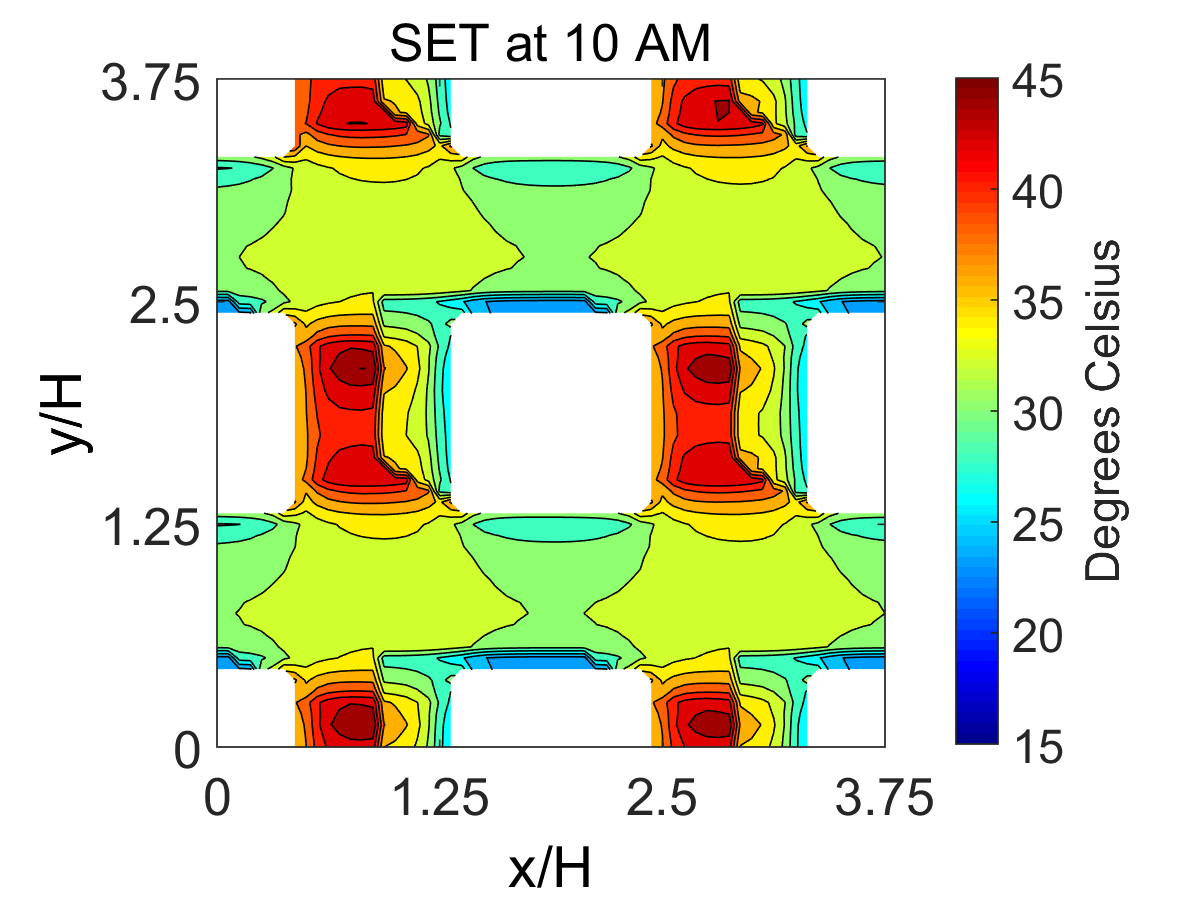
\includegraphics[width=5cm]{SET10AM.png}}} &
&  \\ \cline{1-3}
                       &                       &                       &  &  \\ \cline{1-3}
\multicolumn{1}{|c|}{1200 PST} & \multicolumn{1}{c|}{1400 PST} & \multicolumn{1}{c|}{1800 PST} &  &  \\ \cline{1-3}
\multicolumn{1}{|c|}{\graphicspath{{image/}}\raisebox{-\totalheight}{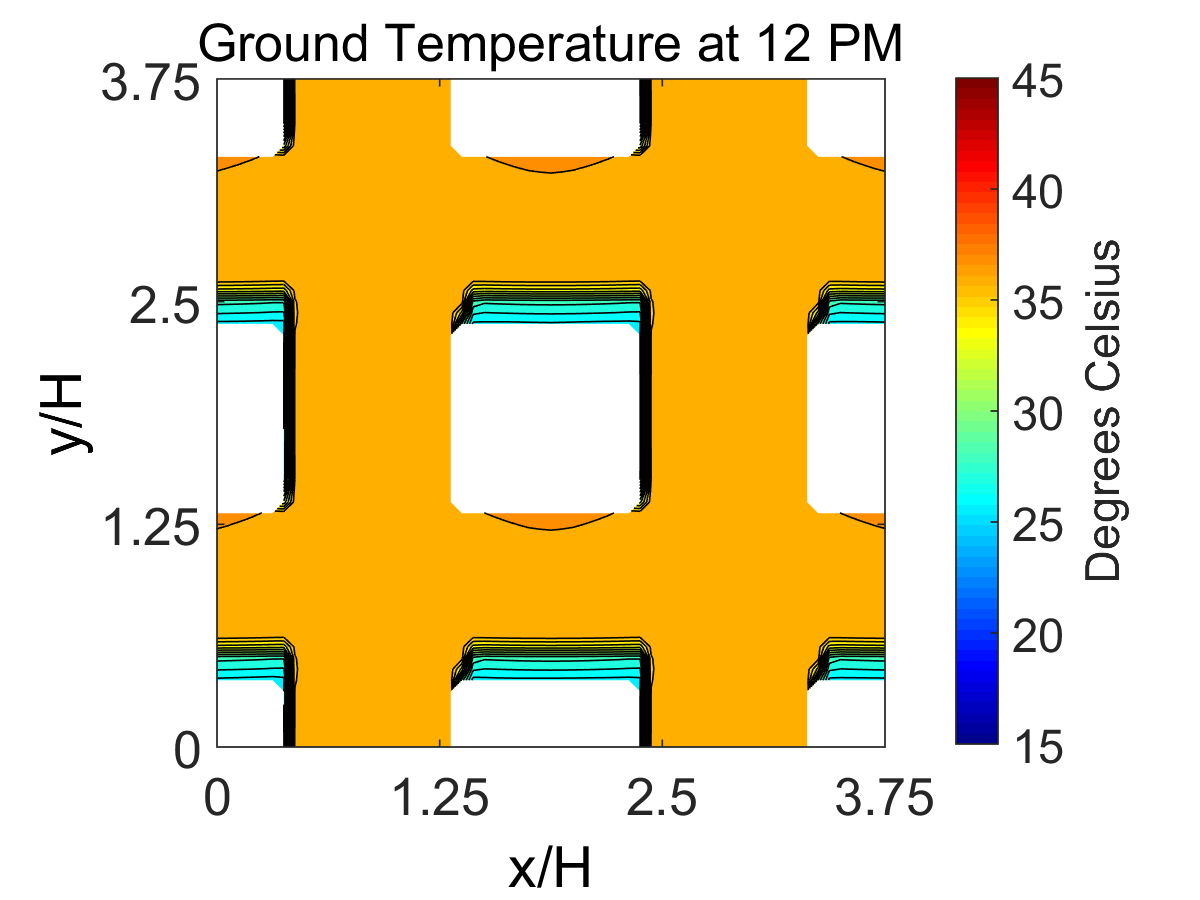
\includegraphics[width=5cm]{Ground12PM.png}}} & 
\multicolumn{1}{c|}{\graphicspath{{image/}}\raisebox{-\totalheight}{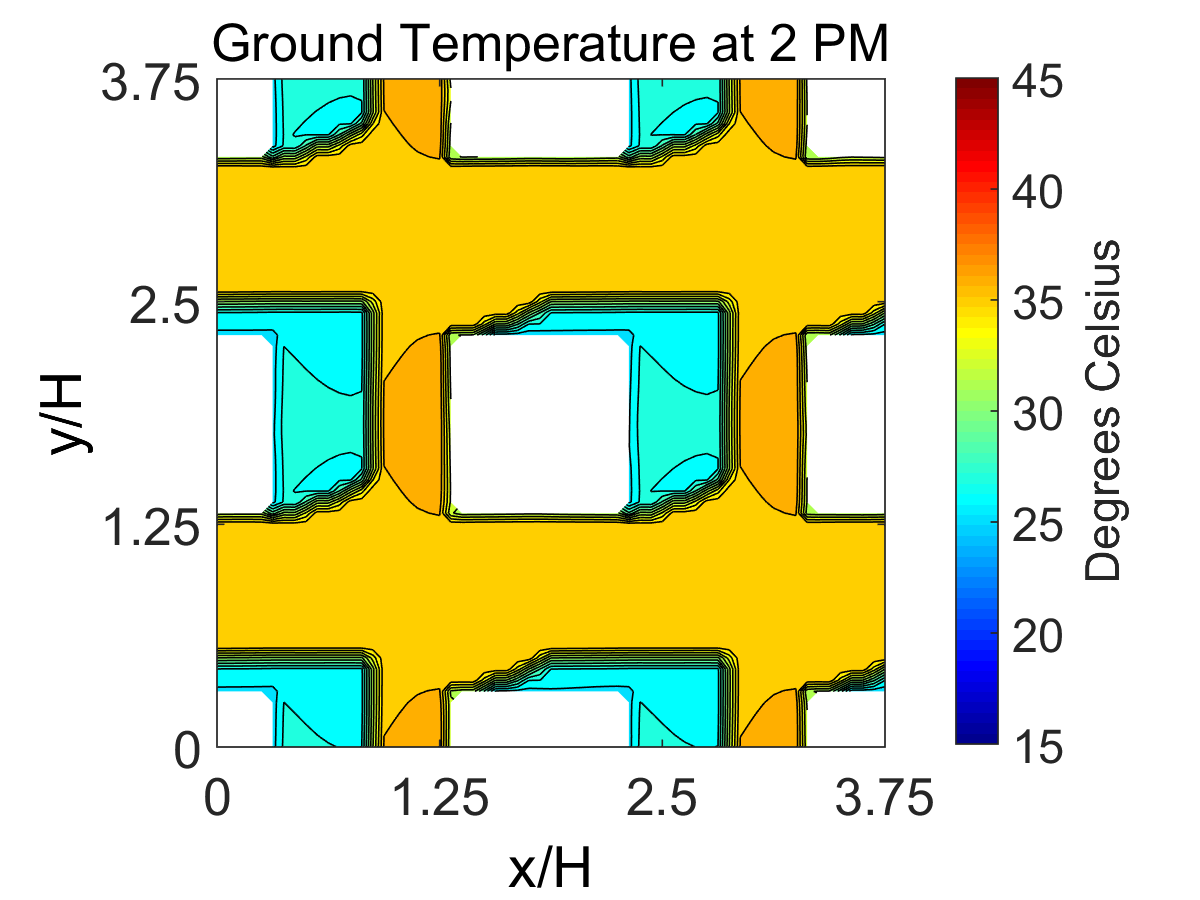
\includegraphics[width=5cm]{Ground2PM.png}}} & 
\multicolumn{1}{c|}{\graphicspath{{image/}}\raisebox{-\totalheight}{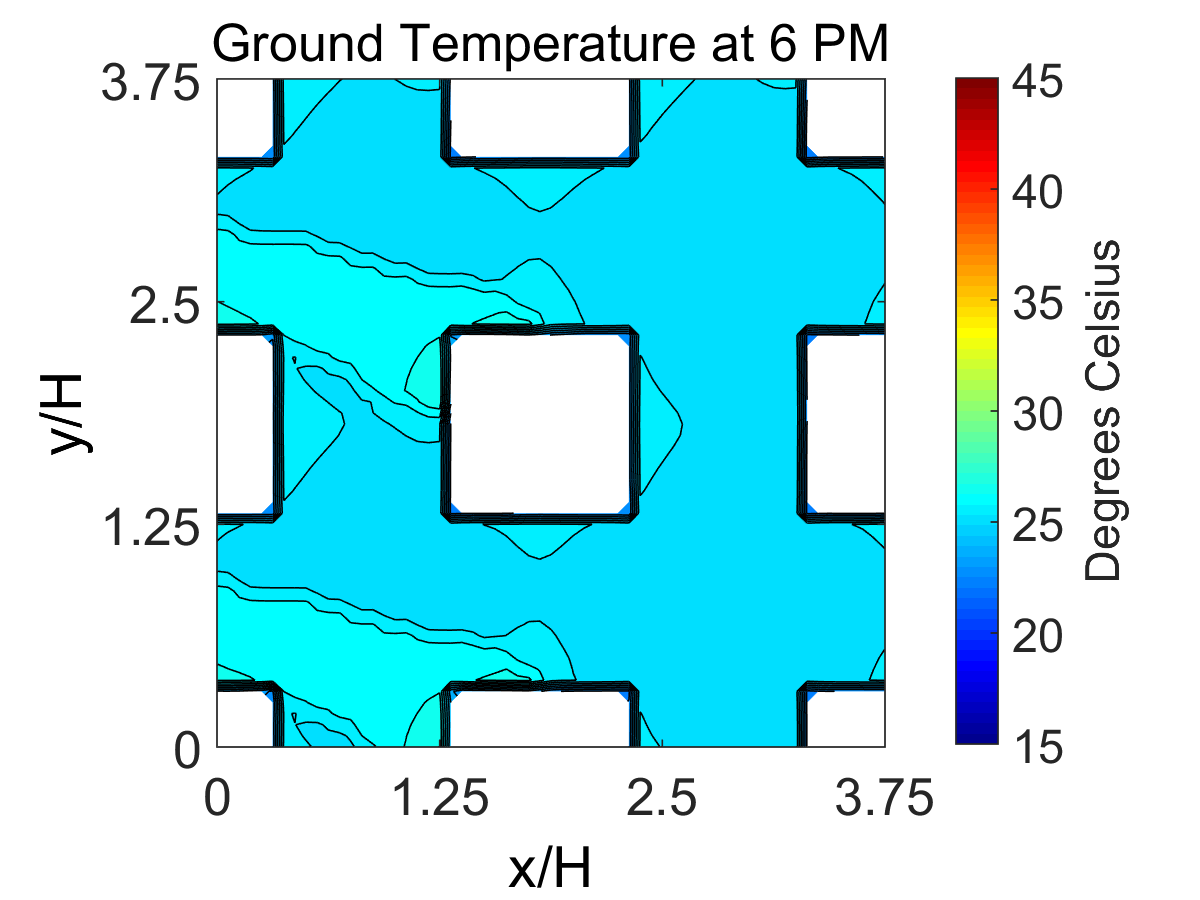
\includegraphics[width=5cm]{Ground6PM.png}}} &  &  \\ \cline{1-3}
\multicolumn{1}{|c|}{\graphicspath{{image/}}\raisebox{-\totalheight}{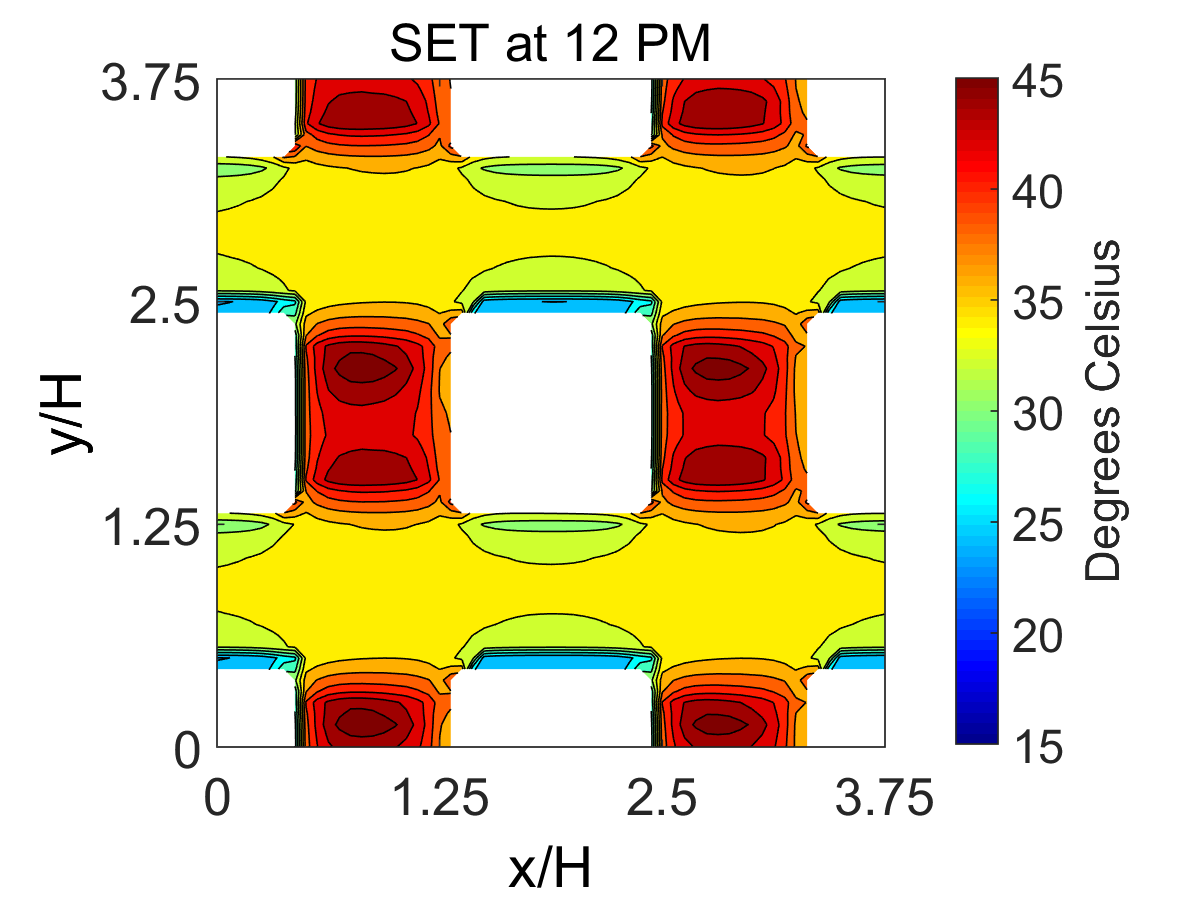
\includegraphics[width=5cm]{SET12PM.png}}} & 
\multicolumn{1}{c|}{\graphicspath{{image/}}\raisebox{-\totalheight}{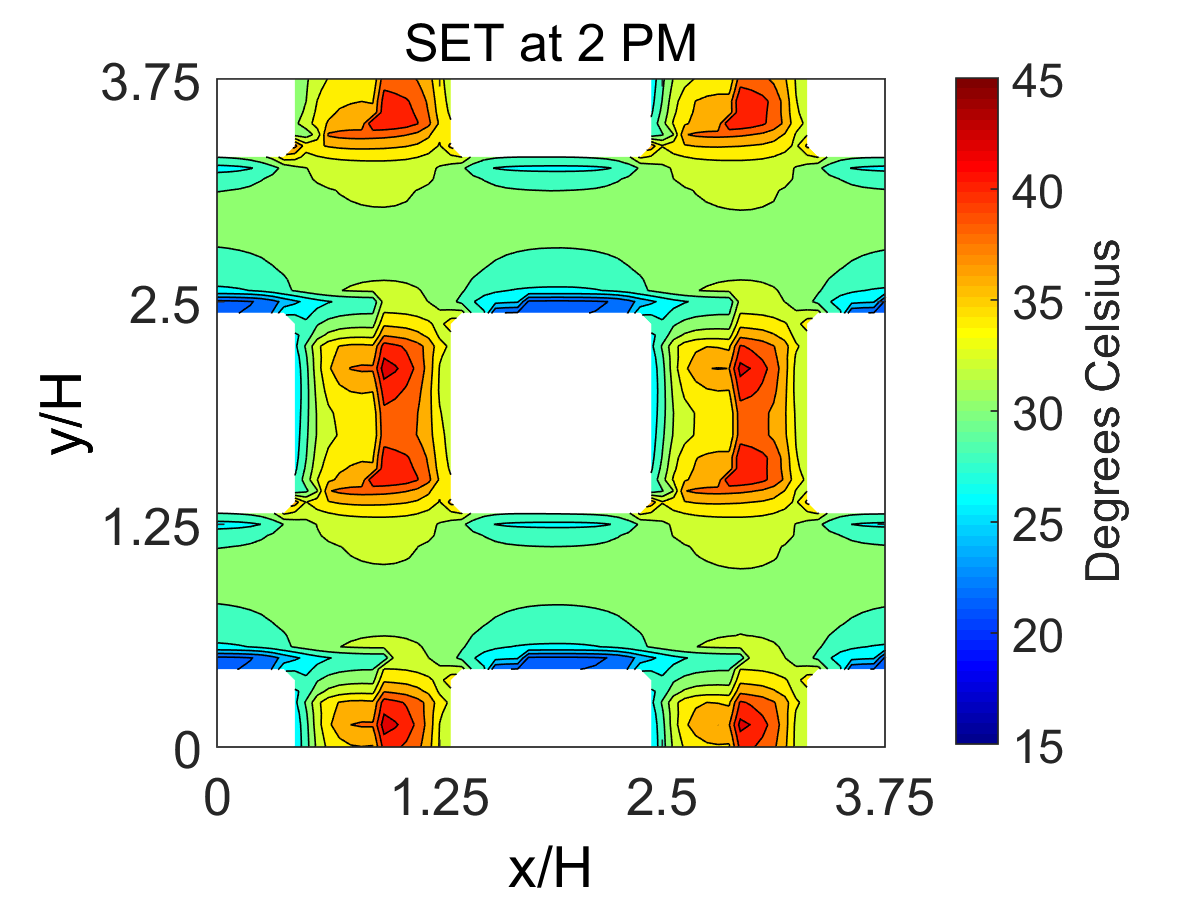
\includegraphics[width=5cm]{SET2PM.png}}} & 
\multicolumn{1}{c|}{\graphicspath{{image/}}\raisebox{-\totalheight}{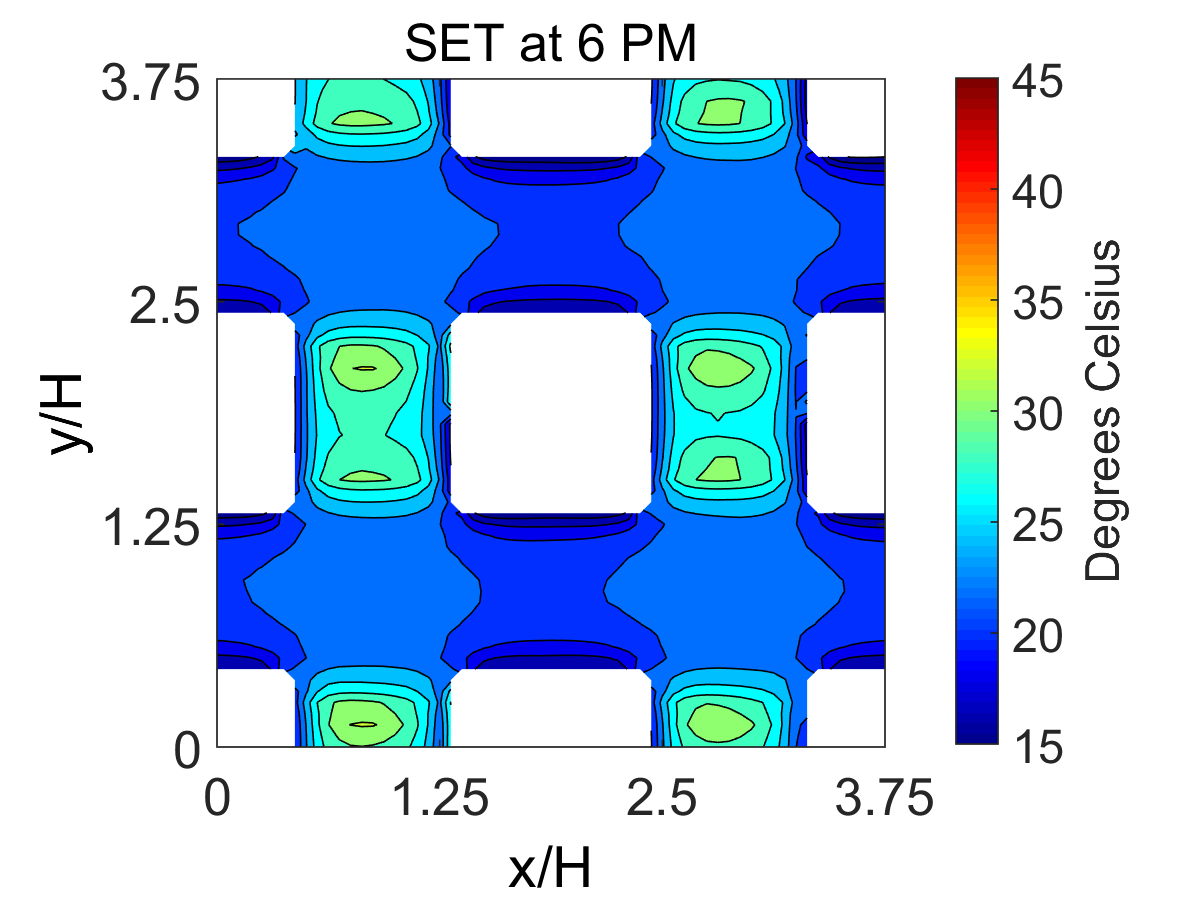
\includegraphics[width=5cm]{SET6PM.png}}} &  &  \\ \cline{1-3}
\end{tabular}
\end{table}


Throughout the day, radiation on the pedestrian changes with the solar angle, while concurrent changes in air temperature and wind flow also influence thermal sensation. For example, shading effects are shown clearly in the comparison between 1000 PST and 1400 PST, in both ground and SET distributions. The importance of shade in mitigating thermal stress can be determined by showing that short-wave radiation is a dominating parameter in SET calculations. 

Air temperature is hottest in the afternoon at 2 PM. However, according to Figure \ref{Fig.SolarIntensity}, the solar peak occurs at noon. From our SET simulation, the SET distribution is hottest at noon, as opposed to 2PM. At noon, the position of the sun minimizes the shading effects of the buildings, and thus, shortwave radiation is dominant. The noontime SET distribution is significantly hotter than in the afternoon, showing that shortwave radiation is more influential in thermal comfort. 
%talk more about location of sun
Nonetheless, the effects of wind flow are still significant. The neutral distribution case isolates the effects of wind flow by calculating SET with uniform surface temperatures. Similarly, the noontime ground temperature distribution is uniform since shading effects are minimal. The effects of wind are apparent in these conditions since the SET distributions show a stark difference between spanwise and streamwise canyons. 



\subsection{Thermal comfort and wind direction}

According to Equation \ref{Eqa.SET}, wind direction is not an explicit variable in SET. However, since wind direction changes the building wall temperature distribution \cite{nazarian2014effects} and air temperature distribution, which are major parameters of SET, it is valuable to analyze the sensitivity of the SET distribution to wind direction. Figure \ref{Fig.NWwind} shows the SET distributions when wind is blown from the northwest and figure \ref{Fig.Swind} shows the wind from the south at PST 1000. The SET distribution shows that wind direction substantially alters the SET distribution. When the wind blows from the south, the SET distribution pattern is very similar to the original 1000 PST distribution from Table \ref{table:DiurnalDist}, only rotated by 90 degrees. When the wind blows from the northwest, the SET distribution pattern is markedly different, despite the identical ground temperature distribution. 


\begin{figure}[H]
\graphicspath{ {image/} }
\centerline{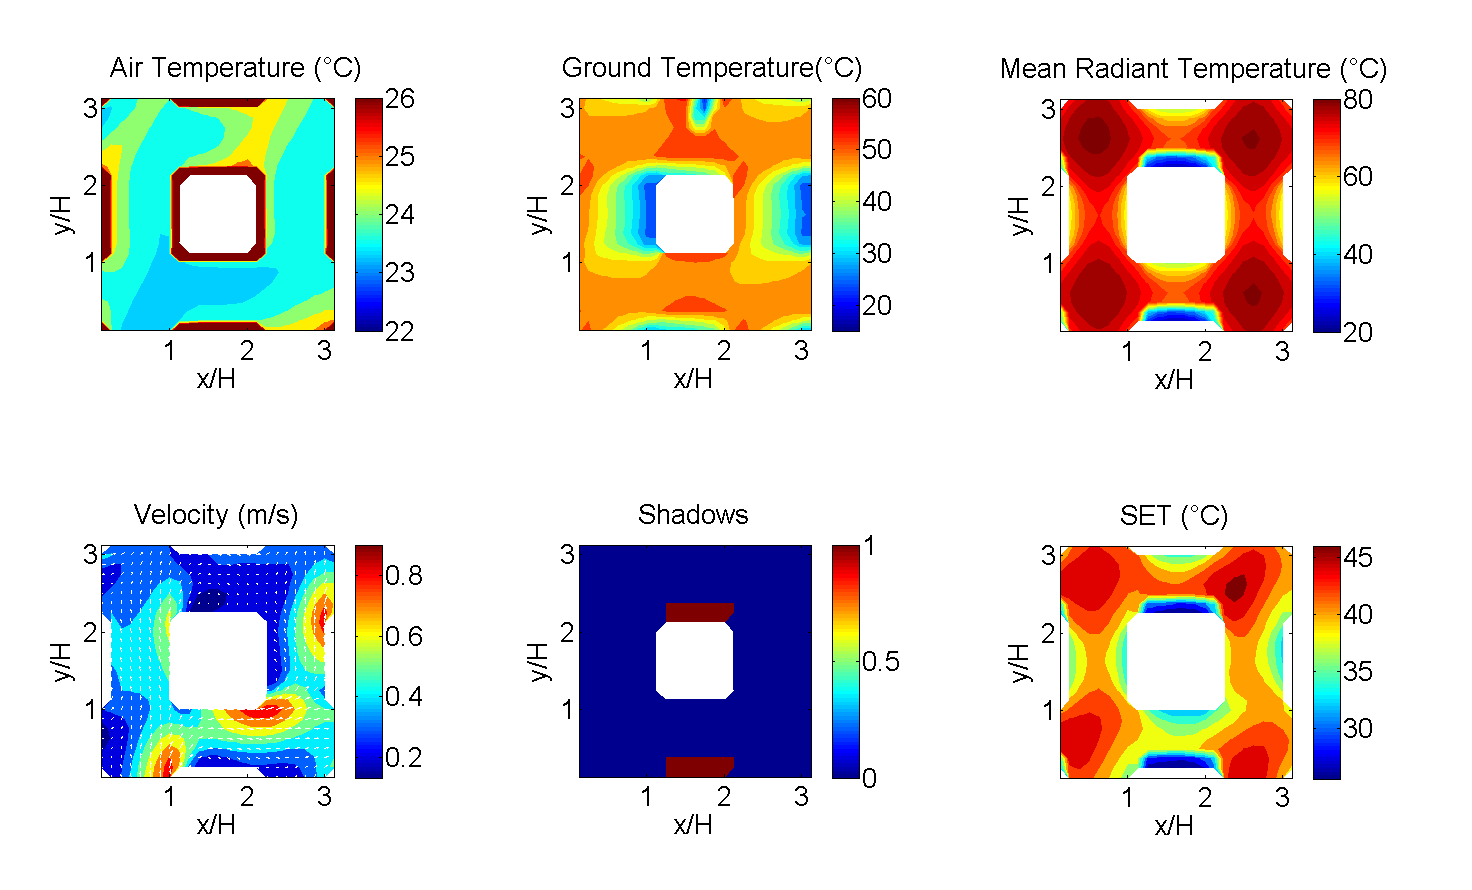
\includegraphics[width=14cm]{936_theta45.png}}    
\caption{Simulation of SET at the pedestrian level as wind blows from the northwest}    
\label{Fig.NWwind}
\end{figure}

\begin{figure}[H]
\graphicspath{ {image/} }
\centerline{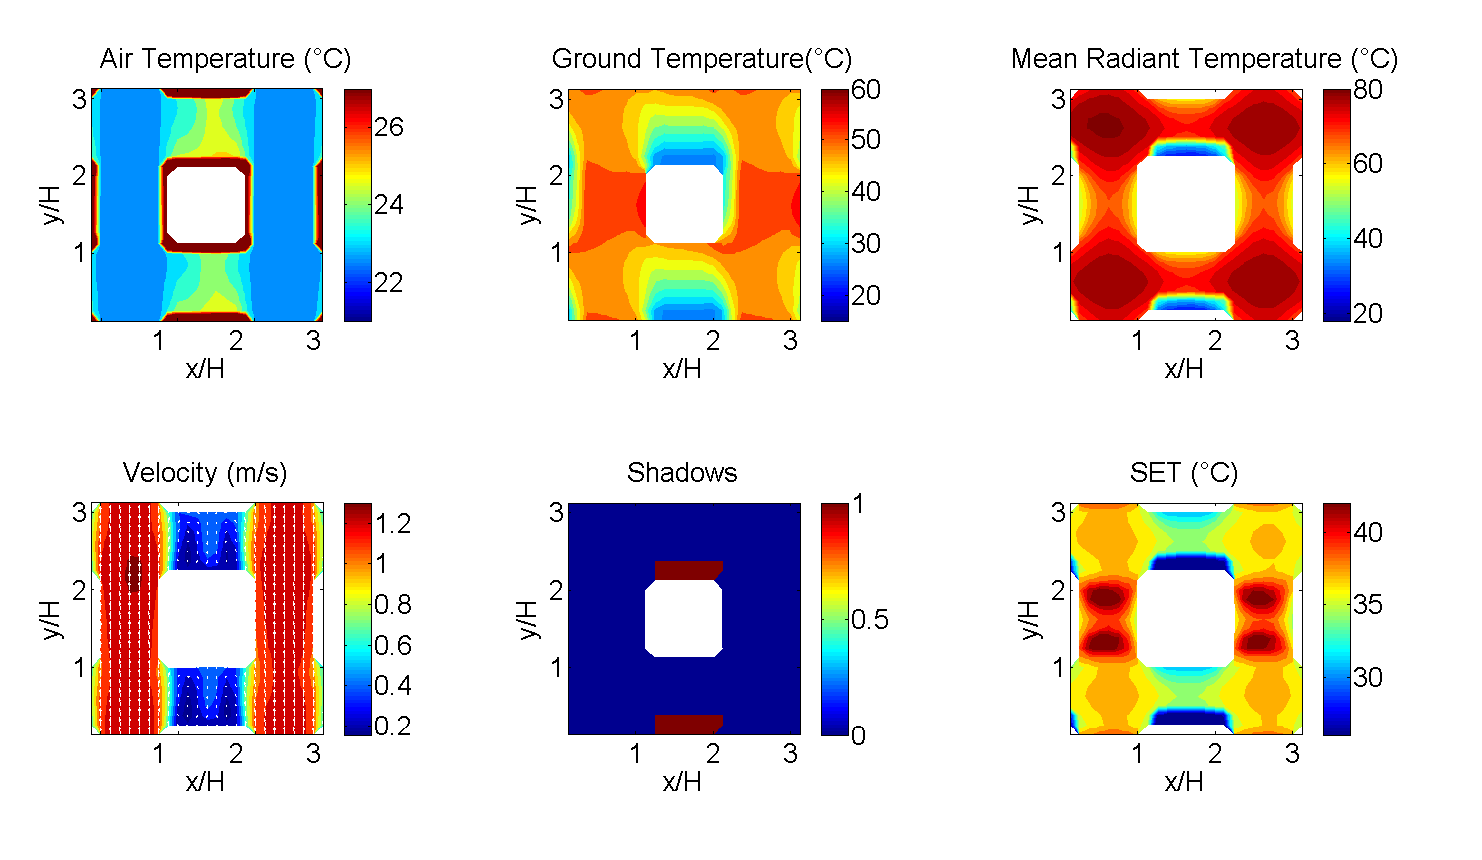
\includegraphics[width=14cm]{theta90.png}}    
\caption{Simulation of SET at the pedestrian level as wind blows from the south}  
\label{Fig.Swind}
\end{figure}


\subsection{Thermal comfort and urban density}

Urban built-up density can be represented in the aspect ratio (AR) of the street canyons, i.e., the ratio of building height to street width (H/W). Street canyon aspect ratio affects both wind flow and shade patterns. In our sensitivity study, the canyon ratio is modified by changing building spacing with constant building height. SET calculations of different aspect ratios were conducted along the same line setup as in Figure \ref{Fig.Line} at 1200 PST. 

\begin{figure}[H]
\graphicspath{ {image/} }
\centerline{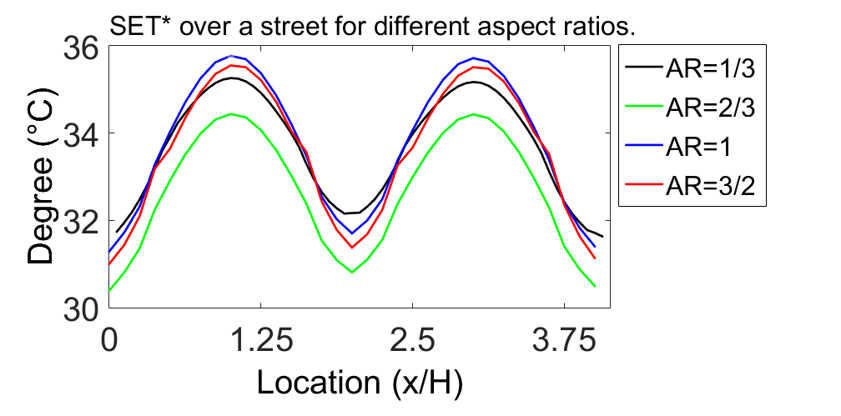
\includegraphics[width=10cm]{ARchange.png}}
\caption{SET distribution change with AR (AR is changed by higher building height therefore the location is referenced by width of buildings W)}
\label{Fig.AR}
\end{figure}

\begin{table}[]
\centering
\caption{Ranges in SET for varying aspect ratios}
\label{table:AR_range}
\begin{tabular}{llll}
  Aspect Ratio  & \textbf{min SET ($^{\circ}$C)} & \textbf{min SET ($^{\circ}$C)} & \textbf{Range ($^{\circ}$C)}\\ \hline
\multicolumn{1}{l|}{\textbf{1:3}} &     32.2      &     35.2      &   3.0        \\
\multicolumn{1}{l|}{\textbf{2:3}} &      30.8     &     34.4      &  3.6         \\
\multicolumn{1}{l|}{\textbf{1:1}} &      31.7     &     35.7      &   4.0       \\
\multicolumn{1}{l|}{\textbf{3:2}} &      31.4     &      35.5     &  4.1        
\end{tabular}
\end{table}

Figure \ref{Fig.AR} indicates that SET does not change monotonically with AR. SET is a complex function wherein different parameters concurrently influence SET.  For example, taller buildings and narrower streets (larger aspect ratios) will increase shade cover. At same time, average wind velocity often decreases with higher AR. These concurrent effects are reflected in the SET calculations. These results indicate that building designs can be optimized for outdoor thermal comfort, in order to maximize shade coverage while also maintaining a comfortable breeze.  




%%%%%%%%%%%%%%%%%%%%%%%%%%%%%%%%%%%%%%%%%%%%%%%%%%%%%%%%%%%%%%%%%%%%%%%%%%%%%%%%%%%%%%%%%%%%%%%%%%%%%

\section{Conclusion and Future Perspective}
This study developed a method for high spatial resolution thermal comfort modeling. A comprehensive non-uniform radiant temperature model was incorporated with detailed wind flow and thermal field simulations into a matrix-based urban model. SET* distributions were calculated as an index of thermal comfort. In the sensitivity analysis of the enhanced model, thermal comfort is found to be highly sensitive to wind patterns and radiant temperature. 

SET simulation results have also been compared to the CBE Thermal Comfort Tool \cite{hoyt2013cbe} which is a licensed thermal comfort calculator. Furthermore, individual components of the simulation method have also been verified. Huang \cite{huang2014citycomfort+} verified the $T_{mrt}$ formula used in this paper (Eqn. \ref{Equ.MRT}), which is improved by adding shade, sky view factor and urban surface visibility modeling. 
Nonetheless, the simulation method is still under development and has yet to be compared with measurement data.  To do so, the idealized urban model needs to be adapted to a realistic urban model in order to verify the simulation using measurement data of $T_{mrt}$. Thus, a more complex model should be developed for buildings with complex geometries, in order to simulate factors such as shading effects and sky view factor appropriately.

This work represents a framework that will be further developed to analyze changes in thermal comfort due to design factors, surface materials, and additional local climate factors. In the next phase, the calculation method will be adapted for realistic urban models, validated experimentally, and compared to other thermal prediction methods, such as ENVI-met 3.1 \cite{bruse2004envi}, Rayman 1.2 \cite{matzarakis2007modelling}, CityComfort+ \cite{huang2014citycomfort+} and SOLWEIG 2.2 \cite{lindberg2008solweig}. 
	

With accurate and detailed thermal comfort predictions, urban planners and architects are better equipped to understand their designs in the context of the local climate and its effects on the urban population. Subsequent analyses can then help to propose necessary strategies to mitigate environmental impacts and health concerns due to the built environment. 



%%%%%%%%%%%%%%%%%%%%%%%%%%%%%%%%%%%%%%%%%%%%%%%%%%%%%%%%%%%%%%%%%%%%%%%%%%%%%%%%%%%%%%%%%%%%%%%%%%%%%

\section{Reference}

\bibliographystyle{plain}
\bibliography{reference}

\end{document}


